%-------------------------------------------------------------------------------
%                            BAB IV
%               		HASIL DAN PEMBAHASAN
%-------------------------------------------------------------------------------
% \fancyhf{} 
% \fancyfoot[R]{\thepage}
\chapter{HASIL DAN PEMBAHASAN}
%\thispagestyle{plain} % Halaman pertama bab menggunakan gaya plain

\section{Analisis akuisisi data}

Dalam penelitian ini, data citra udara hasil tangkapan drone beserta koordinat asli lapangan atau Ground Control Points (GCP) telah diakuisisi oleh staf ahli dari Laboratorium Terpadu Sistem Informasi Geografis dan Data Spasial Universitas Syiah Kuala. Fokus penelitian ini adalah analisis terhadap proses akuisisi data citra udara yang dihasilkan oleh drone. Berdasarkan analisis yang telah dilakukan, terdapat beberapa poin penting yang dapat diuraikan mengenai langkah-langkah akuisisi data tersebut.

\subsection{Desain jalur terbang \textit{drone}}

Dalam proses akuisisi data citra udara menggunakan drone, desain jalur terbang merupakan tahapan yang sangat krusial. Signifikansi desain ini terletak pada pengaruhnya terhadap kualitas citra yang dihasilkan dan efisiensi waktu yang diperlukan untuk menyelesaikan misi penerbangan. Beberapa aspek penting harus dipertimbangkan dalam merancang jalur terbang yang optimal. Pertama, perhitungan cermat mengenai daya tahan baterai sangat diperlukan untuk memastikan cakupan area yang direncanakan dapat terpenuhi dengan satu baterai penuh. Kedua, perencanaan rute harus mampu mencakup seluruh area target yang telah ditentukan sebelumnya. Ketiga, faktor lingkungan seperti arah angin merupakan elemen krusial yang harus diperhitungkan. Penerbangan melawan arah angin akan mengonsumsi daya lebih besar, sehingga dapat mempercepat habisnya baterai selama proses akuisisi data. Dengan mempertimbangkan faktor-faktor tersebut, desain jalur terbang yang optimal dapat menghasilkan citra berkualitas tinggi sekaligus mengoptimalkan penggunaan sumber daya drone, terutama dalam hal konsumsi baterai dan waktu penerbangan.

Dalam proses akuisisi data lahan Kampus II Universitas Syiah Kuala, perencanaan jalur terbang didesain menggunakan perangkat lunak Drone Deploy. Aplikasi ini memungkinkan pengaturan area yang akan dilewati drone, konfigurasi bentuk jalur terbang, serta penyesuaian front overlap dan side overlap antar foto. Selain itu, perangkat lunak ini juga menyediakan estimasi waktu penerbangan dan penggunaan daya baterai drone untuk setiap misi. Penulis telah melakukan analisis perbandingan antara jalur terbang dominan vertikal dan dominan horizontal untuk menentukan efisiensi waktu dan penggunaan daya. Kedua jalur terbang ini dapat dilihat pada Gambar \ref{jalur terbang 1} dan \ref{jalur terbang 2}, sementara perbandingan detailnya disajikan dalam Tabel \ref{tab:perbandingan_jalur}.

\begin{figure}[H]
    \centering
    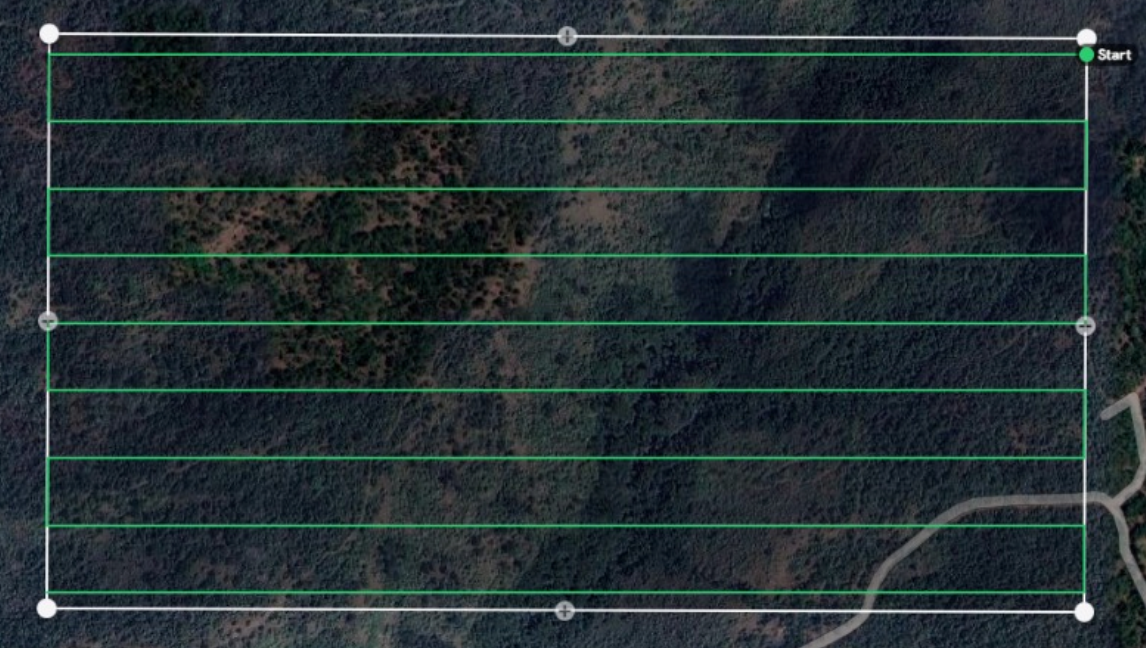
\includegraphics[width = 11.5cm]{image/desain jalur terbang 1.PNG}
    \caption{Jalur terbang dominan horizontal}
    \label{jalur terbang 1}
\end{figure}

\begin{figure}[H]
    \centering
    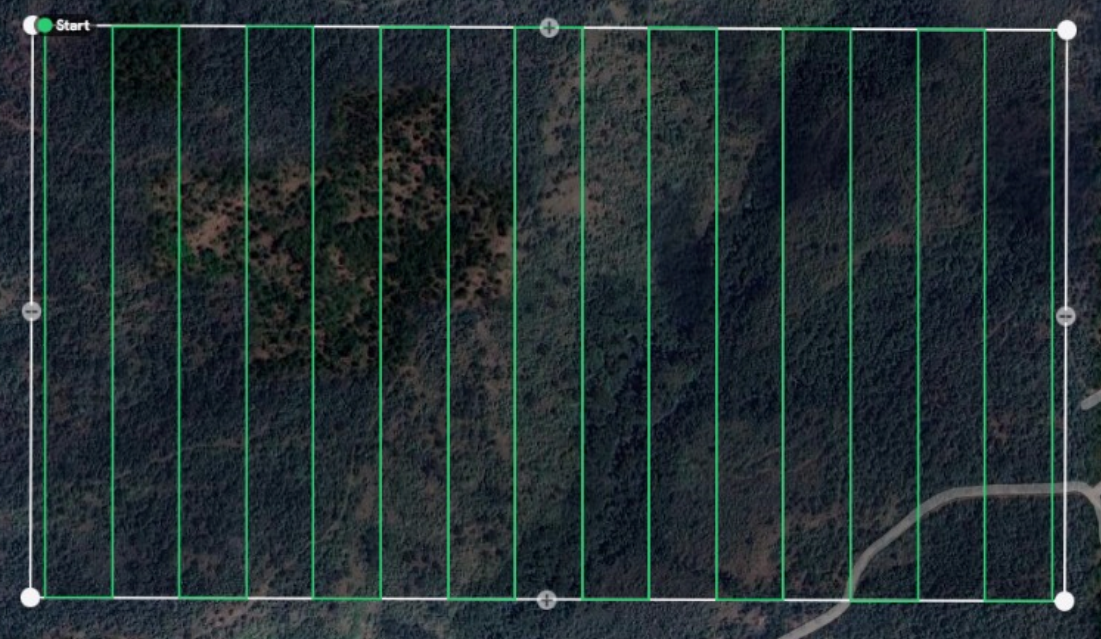
\includegraphics[width = 11.5cm]{image/desain jalur terbang 2.PNG}
    \caption{Jalur terbang dominan vertikal}
    \label{jalur terbang 2}
\end{figure}

\begin{table}[h]
\centering
\caption{Perbandingan jalur terbang dominan vertikal dan horizontal}
\begin{tabular}{|c|c|c|c|c|c|c|}
\hline
\textbf{No} & \textbf{\begin{tabular}[c]{@{}c@{}}Jalur\\terbang\end{tabular}} & \textbf{\begin{tabular}[c]{@{}c@{}}Luas\\Area (H)\end{tabular}} & \textbf{\begin{tabular}[c]{@{}c@{}}Jumlah\\Gambar\end{tabular}} & \textbf{\begin{tabular}[c]{@{}c@{}}Kecepatan\\terbang\\(m/s)\end{tabular}} & \textbf{Baterai} & \textbf{\begin{tabular}[c]{@{}c@{}}Waktu\\(menit)\end{tabular}} \\
\hline
1 & \begin{tabular}[c]{@{}c@{}}Dominan\\Vertikal\end{tabular} & 55 & 283 & 12 & 2 & 18:20 \\
\hline
2 & \begin{tabular}[c]{@{}c@{}}Dominan\\Horizontal\end{tabular} & 55 & 288 & 12 & 2 & 16:46 \\
\hline
\end{tabular}
\label{tab:perbandingan_jalur}
\end{table}

Berdasarkan hasil analisis yang disajikan dalam Tabel \ref{tab:perbandingan_jalur}, dapat ditarik beberapa kesimpulan penting. Pertama, jalur terbang dominan horizontal menunjukkan efisiensi yang lebih tinggi dibandingkan dengan jalur dominan vertikal. Hal ini tercermin dari kemampuannya untuk mengambil jumlah gambar yang lebih banyak (288 dibandingkan 283) dalam waktu yang lebih singkat (16:46 menit berbanding 18:20 menit). Selain itu, analisis ini juga mengungkapkan korelasi antara frekuensi belokan drone dengan durasi misi. Semakin sering drone harus berbelok untuk mencapai jalur pengambilan foto utama, semakin lama waktu yang dibutuhkan untuk menyelesaikan pemetaan area tersebut. Hal ini menjelaskan mengapa jalur dominan horizontal, yang umumnya memiliki lebih sedikit belokan, dapat menyelesaikan misi dengan lebih cepat. Temuan-temuan ini memberikan wawasan berharga untuk optimalisasi perencanaan jalur terbang drone dalam misi pemetaan, dengan implikasi signifikan terhadap efisiensi waktu dan produktivitas pengambilan data.

\subsection{ketinggian dan kecepatan terbang}

Penelitian ini dilakukan di lahan Kampus II Universitas Syiah Kuala, tepatnya di Kecamatan Mesjid Raya, Kabupaten Aceh Besar. Karakteristik area penelitian berupa perbukitan dengan vegetasi lebat, yang menjadi tantangan tersendiri dalam melakukan pemetaan menggunakan drone. Dalam konteks pemetaan drone, ketinggian terbang merupakan faktor krusial yang harus dipertimbangkan dengan cermat. Terdapat hubungan berbanding terbalik antara ketinggian terbang dengan detail dan cakupan area foto, semakin rendah drone terbang, semakin tinggi detail yang dapat ditangkap oleh kamera drone, namun semakin sempit area yang tercakup dalam sebuah foto. Sebaliknya, semakin tinggi ketinggian terbang drone, semakin rendah detail yang dapat ditampilkan, tetapi semakin luas area yang dapat dicakup dalam satu foto. Untuk penelitian ini, ketinggian terbang drone ditetapkan pada 150 meter di atas permukaan tanah, menyeimbangkan kebutuhan detail dan cakupan area.

Selain ketinggian, kecepatan terbang drone juga merupakan parameter penting yang perlu dioptimalkan saat pengambilan foto udara. Kecepatan drone tidak hanya mempengaruhi durasi misi, tetapi juga berdampak signifikan terhadap kualitas gambar yang dihasilkan. Dalam kondisi pencahayaan rendah, drone perlu bergerak lebih lambat untuk menghasilkan gambar yang detail. Hal ini disebabkan oleh penyesuaian shutter speed kamera drone terhadap kondisi cahaya yang minim, mengakibatkan proses pengambilan foto menjadi lebih lambat. Jika drone bergerak terlalu cepat dalam kondisi ini, hasil foto cenderung akan terlihat blur. Sebaliknya, dalam kondisi pencahayaan yang optimal, seperti pada siang hari, drone dapat bergerak lebih cepat. Hal ini dimungkinkan karena shutter speed kamera drone dapat bekerja lebih efisien berkat cahaya yang cukup, sehingga mampu menghasilkan gambar yang tetap tajam dan minim blur meskipun pada kecepatan tinggi. Dalam penelitian ini, proses akuisisi data dilaksanakan pada siang hari dengan kondisi pencahayaan yang optimal. Oleh karena itu, kecepatan terbang drone dapat diatur lebih tinggi, yaitu pada 12 m/s, yang terbukti mampu menghasilkan gambar dengan ketajaman dan detail yang sangat baik.

\subsection{overlapping}

Dalam proses akuisisi data citra resolusi tinggi di kawasan Kampus II Universitas Syiah Kuala, penelitian ini menggunakan komposisi front overlap sebesar 75\% dan side overlap 65\%. Pengaturan ini berada dalam rentang optimal untuk pemetaan fotogrametri menggunakan drone, memastikan kontinuitas data spasial dan memungkinkan rekonstruksi 3D yang akurat. Pemilihan nilai overlapping ini didasarkan pada beberapa pertimbangan, termasuk karakteristik terrain kampus yang beragam dengan area berbukit dan bervegetasi lebat, kebutuhan akan akurasi data tinggi, kompensasi terhadap potensi ketidakstabilan drone akibat faktor lingkungan, serta keseimbangan antara kualitas data dan efisiensi operasional.

Meskipun pengaturan ini terbukti efektif untuk sebagian besar area kampus, beberapa tantangan ditemui di zona dengan vegetasi sangat rapat, menunjukkan perlunya pertimbangan untuk meningkatkan overlap di area-area khusus pada penelitian mendatang. Secara keseluruhan, penggunaan front overlap 75\% dan side overlap 65\% terbukti efektif dalam menghasilkan data spasial yang detail dan akurat, memenuhi tujuan pemetaan kawasan Kampus II Universitas Syiah Kuala.

\subsection{Pengambilan \textit{Ground Control Point} (GCP)}

Proses akuisisi data Ground Control Point (GCP) dalam penelitian ini dilakukan menggunakan GPS Geodetik Hi-Target, yang dikenal dengan akurasinya yang tinggi. Sejumlah 16 titik GCP ditetapkan, yang dikategorikan sebagai 3D GCP karena mencakup data longitude, latitude, dan altitude, memberikan referensi spasial yang komprehensif untuk studi kasus area seluas 250 hektar. Strategi penempatan GCP dirancang dengan cermat, dengan satu titik GCP ditempatkan untuk setiap misi penerbangan drone, memastikan cakupan yang merata dan representatif di seluruh area penelitian. Untuk memudahkan identifikasi GCP dalam citra udara, setiap titik ditandai di lapangan menggunakan terpal berwarna merah berbentuk X, seperti yang diilustrasikan pada Gambar 4.4. Pemilihan lokasi GCP dilakukan dengan pertimbangan khusus, dengan preferensi pada area terbuka yang minim vegetasi untuk memaksimalkan visibilitas dan meminimalkan potensi gangguan sinyal GPS. Penempatan strategis ini tidak hanya memfasilitasi deteksi yang akurat dalam citra drone tetapi juga memastikan kualitas sinyal GPS yang optimal selama pengukuran.

Selain proses pengambilan, data GCP sangat penting dalam proses pembuatan peta yang akurat. GCP berfungsi seperti titik-titik acuan yang lokasinya diketahui dengan pasti di lapangan. Cara kerjanya adalah dengan membandingkan lokasi GCP yang diukur di lapangan menggunakan GPS akurat, dengan lokasi yang sama yang terlihat di foto drone. Melalui perbandingan ini, posisi dan bentuk foto-foto drone dapat diperbaiki agar sesuai dengan kenyataan di lapangan. Proses ini disebut georeferensi dan ortorektifikasi. Hasilnya adalah sebuah peta foto (orthomosaic) yang tidak hanya terlihat bagus, tapi juga akurat secara posisi. Keakuratan ini sangat penting karena membuat peta dapat digunakan bersama dengan data-data peta lainnya tanpa ada masalah perbedaan posisi. Misalnya, peta ini dapat digabungkan dengan peta jalan atau peta bangunan yang sudah ada sebelumnya.

\section{Pengumpulan Data}

Dalam penelitian ini, penulis tidak melakukan akuisisi data foto udara lahan Kampus II Universitas Syiah Kuala secara langsung. Hal ini dikarenakan data foto udara dan data pendukung spasial lainnya telah disediakan dan diakuisisi sebelumnya oleh staf Laboratorium Sistem Informasi Geografis dan Data Spasial Universitas Syiah Kuala. Peran penulis dalam tahap ini terbatas pada pengumpulan dan penyusunan data yang diberikan ke dalam struktur folder yang sistematis, guna memudahkan proses pengolahan dan mosaik di tahap selanjutnya. Dataset yang diperoleh terdiri dari 4.701 foto udara hasil tangkapan drone DJI Phantom 4 Pro. Selain itu, data pendukung spasial lainnya juga disertakan, meliputi data koordinat 3D Ground Control Points (GCP) dalam format XYZ, serta data batas administrasi lahan Kampus II USK dan area studi penelitian. Untuk memberikan gambaran visual, contoh hasil tangkapan drone dapat dilihat pada Gambar \ref{pengda}, sementara data GCP disajikan dalam Tabel \ref{tab:gcp_data}.

\begin{figure} [H]
    \centering
    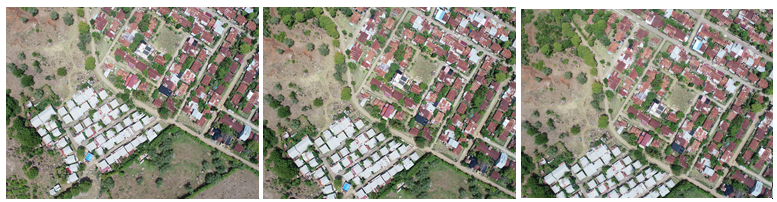
\includegraphics[width=1\linewidth]{image/data.png}
    \caption{Data foto udara \textit{drone}}
    \label{pengda}
\end{figure}

\begin{table} [H]
\centering
\caption{Data Ground Control Point (GCP) area studi penelitian}
\begin{tabular}{|c|c|c|c|}
\hline
\textbf{Label} & \textbf{Latitude} & \textbf{Longitude} & \textbf{Altitude} \\
\hline
GCP 1 & 5.645281 & 95.42608 & 54.587 \\
GCP 2 & 5.646212 & 95.43401 & 38.432 \\
GCP 3 & 5.646481 & 95.44335 & 9.51 \\
GCP 4 & 5.641528 & 95.43029 & 134.79 \\
GCP 5 & 5.641895 & 95.44016 & 94.559 \\
GCP 6 & 5.642268 & 95.44834 & 24.766 \\
GCP 7 & 5.638084 & 95.42901 & 172.052 \\
GCP 8 & 5.63729 & 95.44009 & 185.723 \\
GCP 9 & 5.636904 & 95.44481 & 160.798 \\
GCP 10 & 5.633782 & 95.42898 & 173.878 \\
GCP 11 & 5.633573 & 95.44081 & 180.413 \\
GCP 12 & 5.633305 & 95.44552 & 167.8 \\
GCP 13 & 5.629193 & 95.43453 & 259.766 \\
GCP 14 & 5.630646 & 95.44323 & 245.943 \\
GCP 15 & 5.626161 & 95.43446 & 265.061 \\
GCP 16 & 5.625719 & 95.44308 & 313.595 \\
\hline
\end{tabular}
\label{tab:gcp_data}
\end{table}

\par Dalam proses pengumpulan data, penulis mengadopsi metode pengorganisasian yang sistematis untuk foto-foto udara. Setiap misi penerbangan drone, yang berjumlah total 16 kali di area studi, direpresentasikan oleh satu folder terpisah. Pendekatan ini memungkinkan penulis untuk dengan mudah mengidentifikasi dan menghitung jumlah foto yang diambil dalam setiap misi penerbangan spesifik. Struktur penyimpanan yang terorganisir ini tidak hanya meningkatkan efisiensi dalam pengelolaan dan analisis data visual, tetapi juga meminimalisir risiko kesalahan dalam pengolahan data. Lebih lanjut, metode ini sangat bermanfaat dalam menghadapi potensi tantangan teknis, seperti memudahkan identifikasi dan isolasi masalah jika terjadi error pada area tertentu. Dengan demikian, penulis dapat dengan cepat menavigasi dan mengelola dataset yang besar, sambil mempertahankan integritas data untuk setiap misi penerbangan, yang sangat penting dalam menjaga kualitas hasil penelitian. detail pembagian folder dan jumlah foto pada setiap misi penerbangan dapat dilihat pada tabel \ref{tab:folder}

\begin{table} [H]
\centering
\caption{Pembagian folder dan detail jumlah foto udara didalamnya}
\begin{tabular}{|l|c|}
\hline
\textbf{Nama Folder} & \textbf{Jumlah Foto Udara} \\ \hline
Folder 1 & 291 \\ \hline
Folder 2 & 295 \\ \hline
Folder 3 & 292 \\ \hline
Folder 4 & 291 \\ \hline
Folder 5 & 297 \\ \hline
Folder 6 & 294 \\ \hline
Folder 7 & 293 \\ \hline
Folder 8 & 293 \\ \hline
Folder 9 & 288 \\ \hline
Folder 10 & 292 \\ \hline
Folder 11 & 296 \\ \hline
Folder 12 & 321 \\ \hline
Folder 13 & 285 \\ \hline
Folder 14 & 291 \\ \hline
Folder 15 & 287 \\ \hline
Folder 16 & 296 \\ \hline
\textbf{Total} & \textbf{4701} \\ \hline
\end{tabular}
\label{tab:folder}
\end{table}

\section{mosaik}

\par Pada tahap mosaik ini, penulis akan melakukan proses mosaik menggunakan dua perangkat lunak yang berbeda, yaitu Agisoft Metashape dan Pix4Dmapper. Tujuan dari penggunaan dua perangkat lunak yang berbeda ini adalah untuk membandingkan hasilnya dan menentukan mana yang akan menghasilkan akurasi dan resolusi yang lebih baik.

\subsection{Agisoft Metashape}

\par Dalam penelitian ini, proses mosaik menggunakan perangkat lunak Agisoft Metashape melibatkan beberapa tahap pemrosesan, yaitu align photo, build point cloud, build model, build texture, build DEM, dan build orthomosaic. Langkah pertama yang harus dilakukan adalah mengimpor seluruh foto udara ke dalam perangkat lunak Agisoft Metashape. Penting untuk memastikan bahwa semua foto udara telah dimasukkan dengan lengkap, tanpa ada satu pun yang tertinggal. Align Photo merupakan tahap awal yang krusial dalam proses menghasilkan orthomosaik dari foto udara yang diambil menggunakan drone. Pada tahap ini, perangkat lunak Agisoft Metashape akan memposisikan foto-foto berdasarkan data koordinat yang terekam saat drone melakukan pemotretan udara. Selain menempatkan foto sesuai dengan data koordinat, perangkat lunak juga mengidentifikasi sudut pengambilan gambar drone terhadap permukaan lahan yang dipotret. Penting untuk memastikan bahwa semua foto telah diatur dengan tepat sebelum melanjutkan ke tahap berikutnya. Hasil dari proses ini berupa titik-titik informasi relatif dari setiap foto dalam ruang tiga dimensi yang dapat dilihat pada Gambar \ref{tiepoint}, yang menjadi dasar untuk tahap-tahap selanjutnya dalam pembuatan orthomosaik.

\begin{figure} [H]
    \centering
    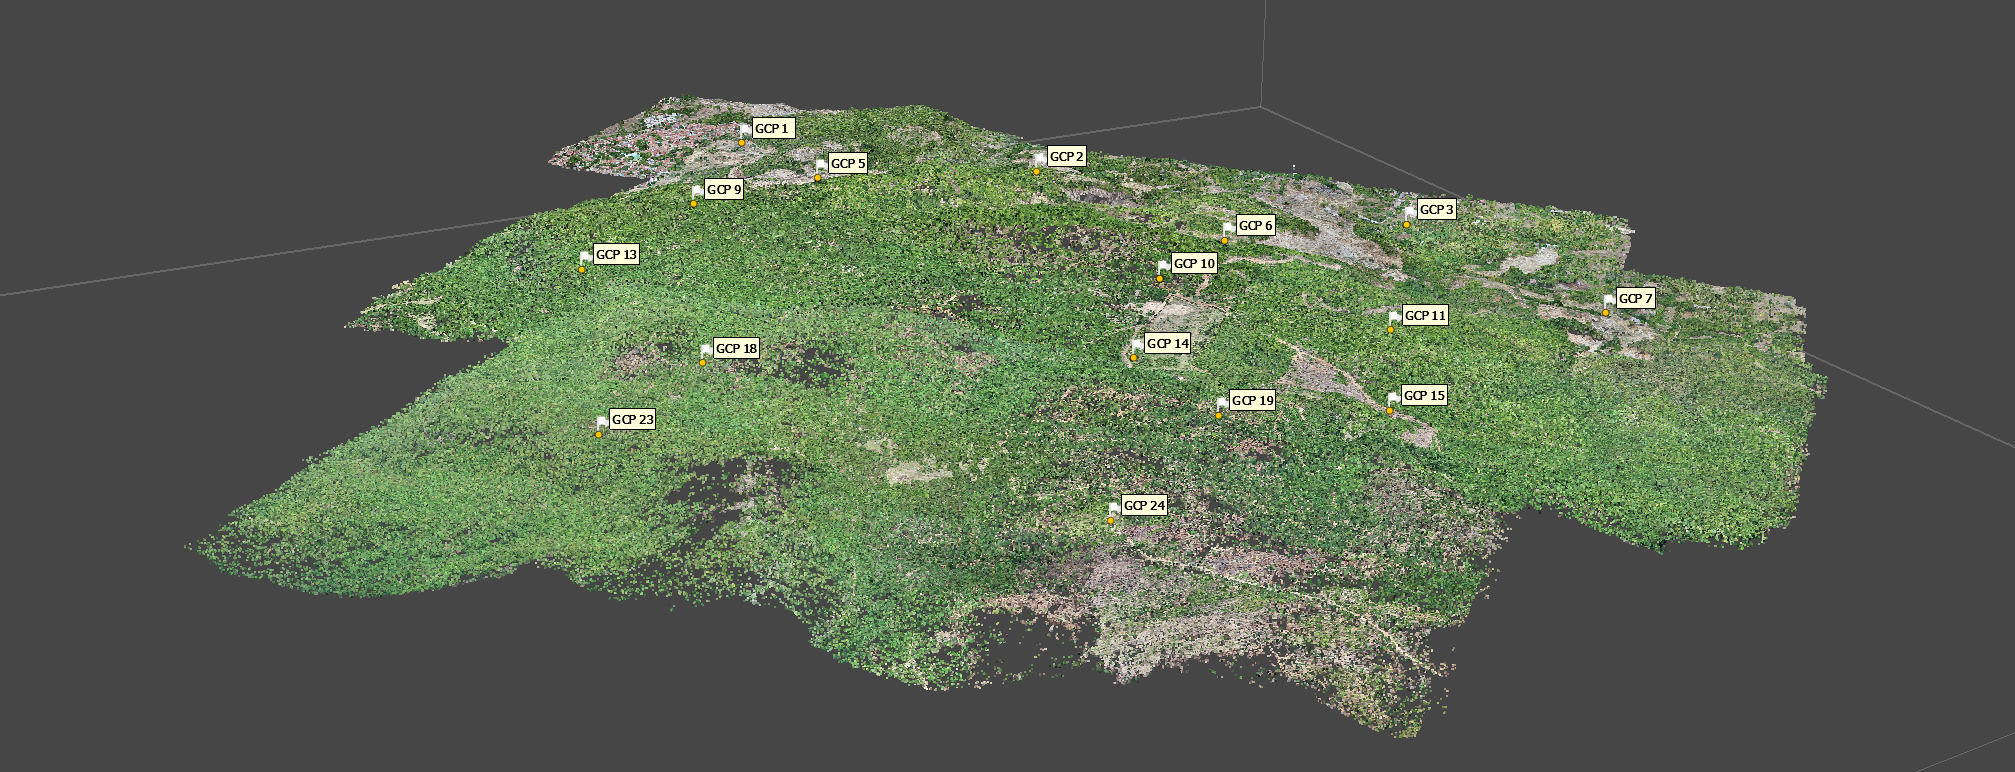
\includegraphics[width=1\linewidth]{image/Tie Point.png}
    \caption{Hasil output dari proses align photo}
    \label{tiepoint}
\end{figure}

Setelah tahap Align Photo berhasil dilaksanakan, langkah berikutnya dalam pemetaan lahan menggunakan drone adalah memasukkan dan menyesuaikan titik Ground Control Point (GCP). Proses ini melibatkan penyelarasan antara koordinat GCP dengan titik-titik yang telah ditandai pada citra hasil tangkapan drone. Dalam penelitian ini, penanda GCP berupa terpal merah berbentuk X digunakan sebagai referensi, seperti yang terlihat pada Gambar \ref{terpal merah}.

\begin{figure} [H]
    \centering
    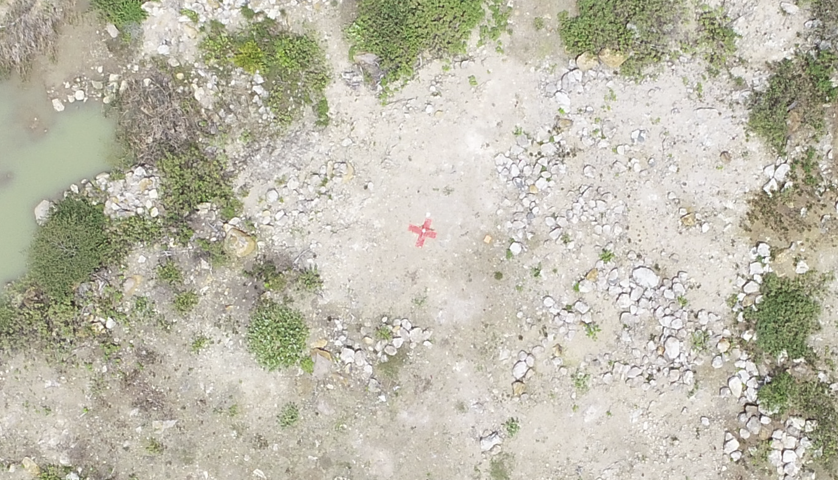
\includegraphics[width = 11.5cm]{image/tanda GCP di lapangan.png}
    \caption{Terpal merah sebagai titik penanda di lapangan}
    \label{terpal merah}
\end{figure}

Penyesuaian koordinat GCP dilakukan dengan teliti pada beberapa citra yang memuat penanda GCP. Berdasarkan tahap pengumpulan data sebelumnya, dataset citra dibagi menjadi 16 folder, masing-masing berisi sekitar 290 gambar dan memiliki satu GCP yang telah ditentukan. Dengan demikian, total GCP yang digunakan dalam proyek ini berjumlah 16 titik. Distribusi spasial dari titik-titik GCP dapat dilihat pada Gambar \ref{penyebaran}. Sementara itu, tahapan penyesuaian koordinat GCP terhadap citra drone diilustrasikan pada Gambar \ref{gcptidakakurat} dan \ref{gcpakurat}, memberikan gambaran visual tentang proses penyelarasan yang dilakukan.

\begin{figure} [H]
    \centering
    \frame{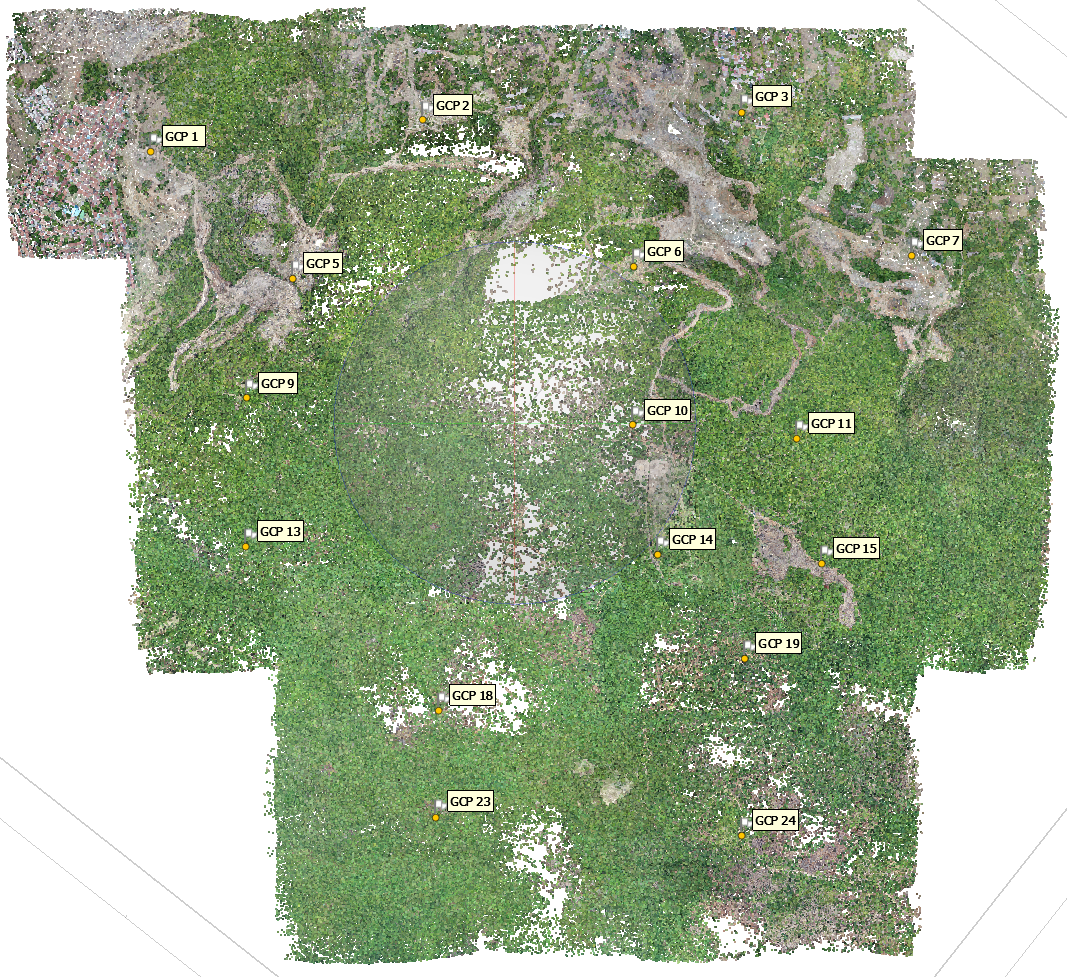
\includegraphics[width=1\linewidth]{image/penyebaran titik GCP - setelah align photo.png}}
    \caption{Penyebaran titik Ground Control Point di area penelitian}
    \label{penyebaran}
\end{figure}

\begin{figure}[H]
    \centering
    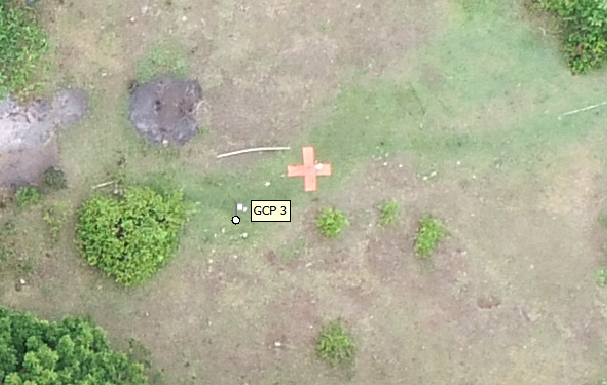
\includegraphics[width = 11.5cm]{image/gcp tidak akurat.png}
    \caption{Titik Ground Control Point sebelum di koreksi}
    \label{gcptidakakurat}
\end{figure}

\begin{figure}[H]
    \centering
    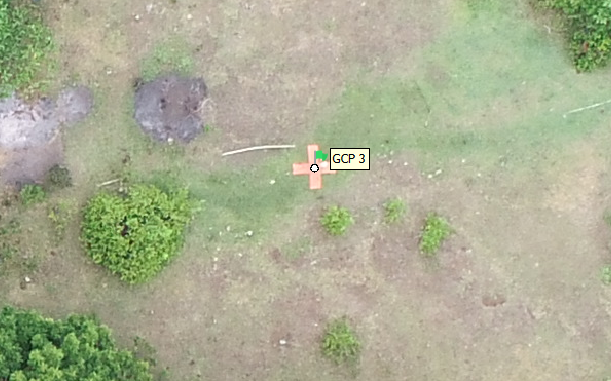
\includegraphics[width = 11.5cm]{image/gcp akurat.png}
    \caption{Titik Ground Control Point setelah di koreksi}
    \label{gcpakurat}
\end{figure}


Tahap selanjutnya adalah Build Point Cloud, sebuah proses yang memerlukan waktu lebih lama dan sumber daya perangkat keras yang paling intensif. Dalam tahap ini, perangkat lunak Agisoft Metashape menghasilkan titik-titik 3D yang secara akurat merepresentasikan permukaan objek atau area lahan yang dipetakan. Perangkat lunak ini memanfaatkan informasi yang diperoleh dari foto-foto yang telah diatur sebelumnya untuk menentukan posisi 3D dari fitur-fitur yang terlihat pada setiap gambar dengan presisi tinggi. Hasil dari proses ini adalah kumpulan titik-titik yang mewakili struktur permukaan yang dipetakan, dengan tingkat kepadatan yang jauh lebih tinggi dibandingkan tie points yang dihasilkan pada tahap Align Photo. Dalam penelitian ini, proses Build Point Cloud memakan waktu 13 jam 48 menit dengan pengaturan kualitas tinggi (High Quality), menghasilkan 1.850.290.607 titik. Visualisasi hasil dari tahap Build Point Cloud dapat dilihat pada Gambar \ref{point cloude}.

\begin{figure} [H]
    \centering
    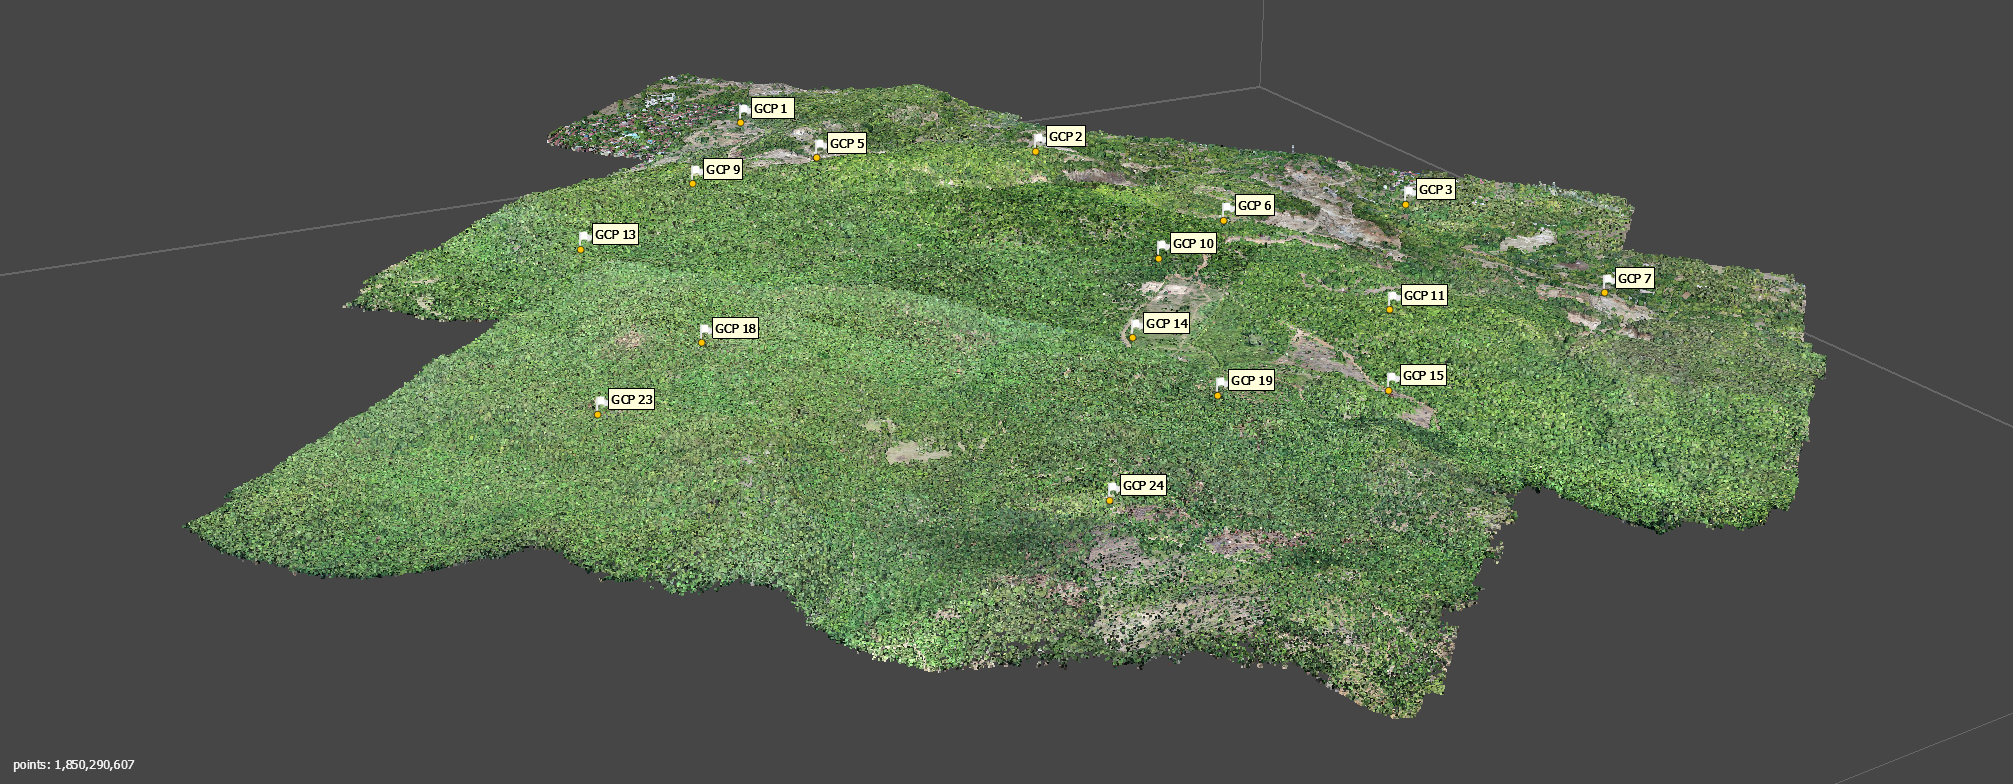
\includegraphics[width=1\linewidth]{image/point cloude.png}
    \caption{Hasil output dari proses build point cloud}
    \label{point cloude}
\end{figure}

\par Setelah point cloud terbentuk, langkah berikutnya adalah membangun model 3D beserta teksturnya. Dalam perangkat lunak Agisoft Metashape, proses ini dapat dijalankan secara terpisah melalui dua tahap yaitu Build Model dan Build Texture. Tahap Build Model menghasilkan model 3D yang solid dan representatif dari objek atau area yang dipetakan. Proses ini menghubungkan titik-titik dari point cloud untuk membentuk permukaan yang mulus dan menghasilkan representasi 3D yang akurat. Hasilnya adalah model 3D yang dapat dilihat dan dimanipulasi. Untuk memperoleh hasil visual yang menarik dan detail yang lebih baik, proses Build Mesh harus dipadukan dengan tahap Build Texture. Pada tahap ini, Agisoft Metashape memetakan kembali gambar-gambar asli dari setiap sudut pengambilan foto ke model 3D. Hasilnya adalah model yang memiliki penampilan realistis dengan warna dan tekstur yang sesuai dengan objek sebenarnya, memberikan visualisasi yang lebih detail dan nyata dari struktur atau area yang dipetakan. Hasil akhir dari proses Build Model dan Build Texture dapat dilihat pada Gambar \ref{model3d}, menampilkan model 3D bertekstur yang menggambarkan area pemetaan dengan tingkat detail dan realisme yang tinggi.

\begin{figure} [H]
    \centering
    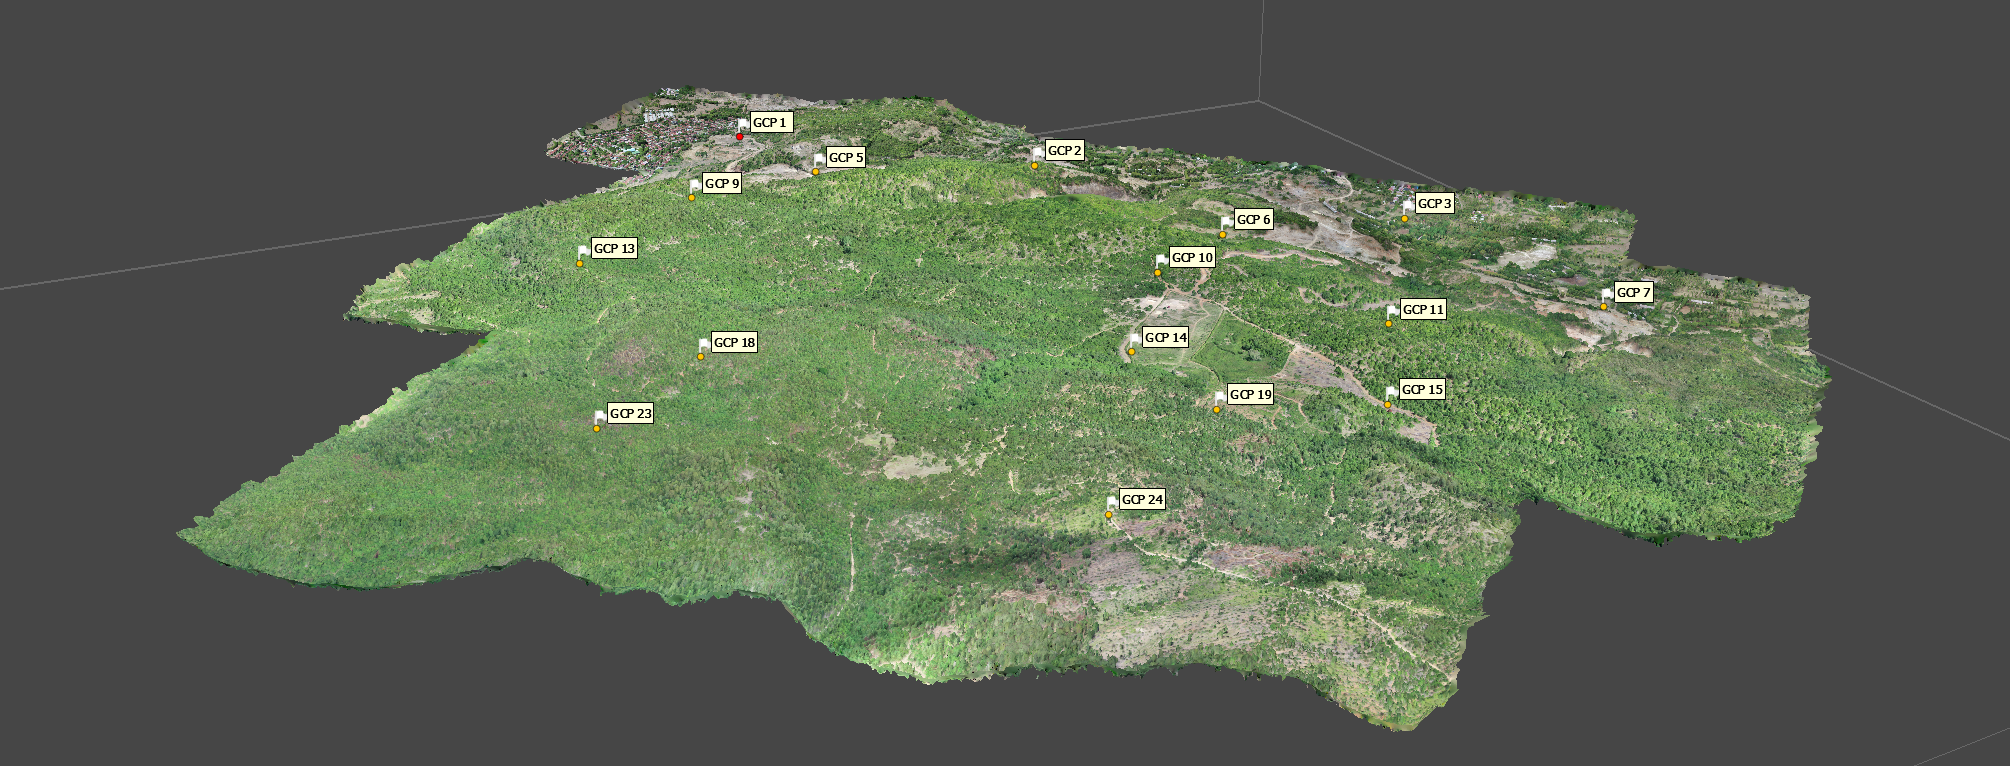
\includegraphics[width=1\linewidth]{image/Tampilan 3d model.png}
    \caption{Hsil output dari proses build model dan build texture}
    \label{model3d}
\end{figure}

\par Setelah proses Build Mesh dan Build Texture berhasil dilaksanakan, langkah selanjutnya adalah membangun Digital Elevation Model (DEM). Tahap ini merupakan proses yang relatif cepat, bahkan dapat selesai dalam hitungan menit. Pada tahap ini, perangkat lunak Agisoft Metashape memanfaatkan data yang telah diolah sebelumnya untuk menghasilkan model digital yang merepresentasikan elevasi permukaan tanah atau objek di area yang dipetakan. DEM yang dihasilkan oleh Agisoft Metashape merupakan output 2D. DEM ini adalah representasi raster dari elevasi permukaan bumi, di mana setiap piksel menyimpan nilai ketinggian tertentu. Meskipun outputnya 2D, DEM ini mampu menggambarkan informasi ketinggian dalam bentuk yang dapat diinterpretasikan sebagai relief permukaan. Output DEM ini biasanya ditampilkan dengan gradasi warna atau bayangan (hillshade) untuk memvisualisasikan perbedaan elevasi. Warna-warna yang berbeda atau intensitas bayangan menunjukkan variasi ketinggian di seluruh area yang dipetakan.

Hasil dari proses Build DEM ini dapat dilihat pada Gambar \ref{dem}, yang menampilkan peta elevasi 2D dari area yang dipetakan, dengan skema warna yang menunjukkan perbedaan ketinggian.
DEM 2D ini tetap sangat berguna untuk berbagai analisis seperti perhitungan kemiringan, aspek, dan kontur, serta dapat digunakan sebagai input untuk analisis perencanaan lahan, dan aplikasi GIS lainnya.

\begin{figure} [H]
    \centering
    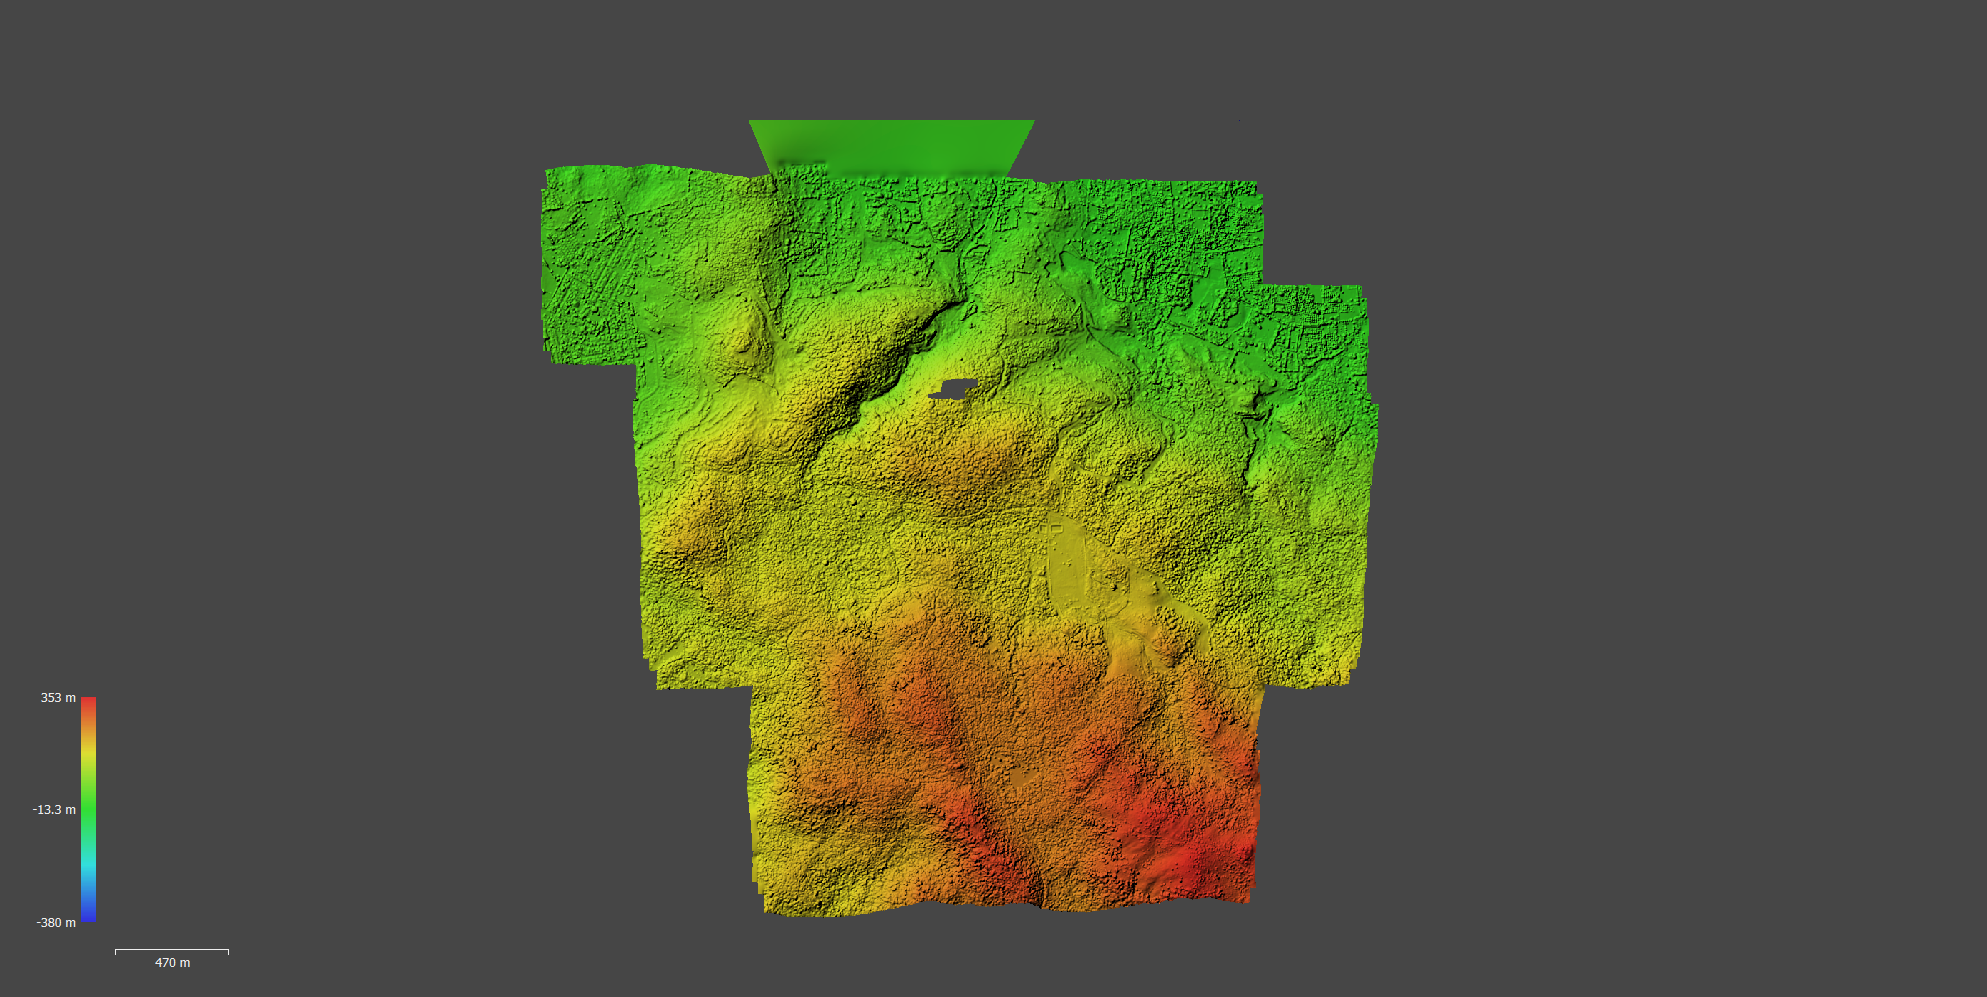
\includegraphics[width=1\linewidth]{image/DEM.png}
    \caption{Hasil output dari proses build Digital Elevation Model (DEM)}
    \label{dem}
\end{figure}

\par Setelah proses Build DEM selesai, tahap terakhir yang dilakukan adalah Build Orthomosaic. Pada tahap ini, perangkat lunak Agisoft Metashape akan menghasilkan ortofoto, yang merupakan citra udara yang telah dikoreksi secara geometris dari area yang dipetakan. Proses ini menggabungkan informasi dari seluruh foto yang telah diatur sebelumnya untuk menciptakan representasi visual yang akurat secara geometris dari wilayah yang diteliti. Hasil akhir dari proses ini adalah orthomosaik, yaitu citra yang memiliki presisi tinggi dari area penelitian, seperti yang ditunjukkan pada Gambar \ref{orthomosaic}. Orthomosaik ini memiliki skala yang konsisten di seluruh gambar, menjadikannya sangat berharga untuk berbagai aplikasi. Data output ini dapat digunakan secara luas dalam pemetaan detail, pemantauan perubahan penggunaan lahan, perencanaan tata ruang, analisis lingkungan, serta berbagai studi dan aplikasi geospasial lainnya yang memerlukan data visual yang akurat secara geometris.

\begin{figure} [H]
    \centering
    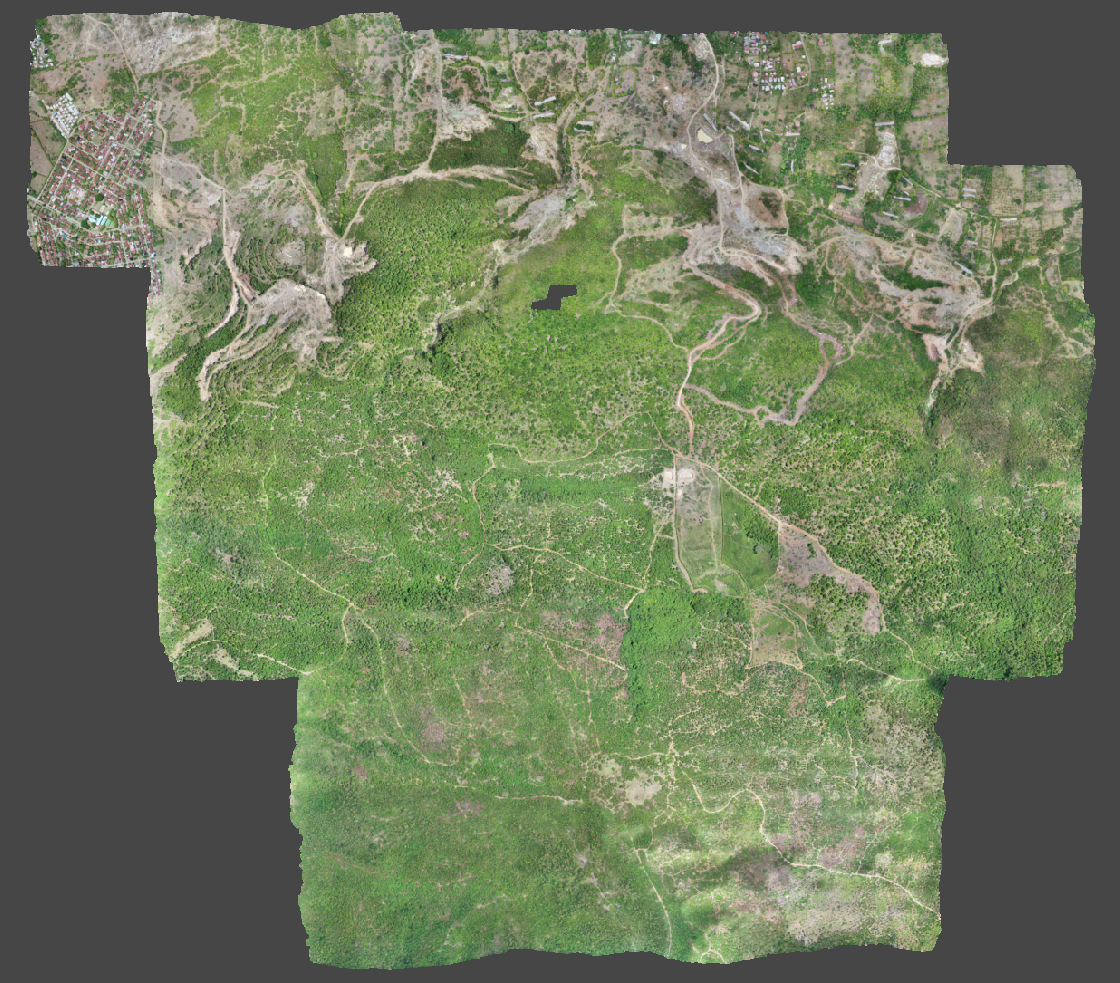
\includegraphics[width=1\linewidth]{image/Orthomosaic.png}
    \caption{Hasil output dari proses build Orthomosaic}
    \label{orthomosaic}
\end{figure}

\par Berdasarkan serangkaian proses mosaik yang telah dilaksanakan, kita memperoleh beberapa hasil, salah satunya adalah gambar orthomosaic. Dalam pelaksanaan proses mosaik menggunakan perangkat lunak Agisoft Metashape, terdapat beberapa kendala di mana pengaturan kualitas tertinggi tidak dapat diimplementasikan secara optimal. Berikut ini, penulis akan memaparkan secara rinci mengenai proses, konfigurasi kualitas, serta durasi yang diperlukan untuk menjalankan setiap tahapan. Informasi tersebut dapat dilihat secara komprehensif pada Tabel \ref{tabel hasil agisoft}.

\begin{table}[H]
\centering
\caption{Ringkasan detail Proses Mosaik menggunakan Agisoft Metashape}
\begin{tabular}{|c|c|c|c|c|}
\hline
\textbf{Proses} & \textbf{Pengaturan} & \textbf{Waktu} & \textbf{Penggunaan} & \textbf{Ukuran} \\
 & \textbf{Kualitas} & \textbf{proses} & \textbf{RAM} & \\
\hline
Align Photo & High & 1 jam 12 menit & 3,07 GB & 345,23 MB \\
\hline
Point Cloud & High & 13 jam 48 menit & 10,99 GB & 23,49 GB \\
\hline
Build Model & Medium & 3 jam 17 menit & 18,35 GB & 5,42 GB \\
\hline
Build Texture & - & 5 jam 52 menit & 14,27 GB & 5,42 GB \\
\hline
Build DEM & Ultra High & 9 menit & 476,43 MB & 4,37 GB \\
\hline
Build Orthomosaic & - & 2 jam 48 menit & 7,33 GB & 112,25 GB \\
\hline
\end{tabular}
\label{tabel hasil agisoft}
\end{table}

\par Data pada Tabel \ref{tabel hasil agisoft} menunjukkan kualitas tertinggi yang dapat diproses oleh spesifikasi komputer penulis. Upaya untuk menjalankan proses dengan kualitas yang lebih tinggi mengakibatkan perangkat lunak mengeluarkan pesan kesalahan "bad allocation". Berdasarkan diskusi dalam komunitas pengguna Agisoft Metashape, hal ini mengindikasikan bahwa komputer yang digunakan tidak memiliki kapasitas RAM yang memadai untuk memproses data sebanyak dan sebesar yang diinputkan. Kesalahan ini dapat terjadi ketika perangkat lunak tidak mampu mengalokasikan jumlah memori yang diperlukan untuk menyelesaikan tugas. Perlu dicatat bahwa hal ini tidak selalu berarti total RAM yang terpasang pada sistem tidak cukup, melainkan lebih kepada jumlah RAM yang tersedia saat operasi tersebut dilakukan. Untuk data dalam tabel yang ditandai dengan simbol (-), hal ini menunjukkan tidak adanya pilihan pengaturan kualitas sebelum proses berjalan dan cenderung menggunakan data olahan sebelumnya. Berdasarkan analisis tabel tersebut, dapat disimpulkan bahwa untuk menjalankan proses mosaik menggunakan Agisoft Metashape dengan data foto udara pada penelitian ini membutuhkan waktu total selama 27 jam 8 menit. Selain itu, dari kolom ukuran dapat diestimasi bahwa untuk menjalankan proyek ini dibutuhkan ruang penyimpanan kosong lebih dari 145,88 GB pada komputer. Informasi ini sangat penting untuk memastikan kesiapan sumber daya komputasi sebelum memulai proyek pengolahan data foto udara yang kompleks.

Selain mempertimbangkan pengaturan kualitas dan waktu pemrosesan yang dibutuhkan, keakuratan geometri merupakan aspek yang sangat penting untuk diperhatikan. Keakuratan ini tidak hanya mempengaruhi kualitas hasil akhir, tetapi juga berimplikasi pada validitas analisis spasial yang akan dilakukan selanjutnya. Untuk mengevaluasi tingkat keakuratan geometri ini, metode yang umum digunakan adalah pengukuran Root Mean Square Error (RMSE) pada Ground Control Points (GCP). Berikut pada Tabel \ref{tab:gcp_error} hasil analisis keakuratan geometri GCP menggunakan metode RMSE, yang memberikan gambaran kuantitatif tentang presisi spasial hasil mosaik.



\begin{table}[h]
\centering
\renewcommand{\arraystretch}{1.2}
\caption{Nilai RMSE dari control point Agisoft Metashape}
\begin{tabular}{|l|r|r|r|r|r|}
\hline
\textbf{Label} & \textbf{X error (cm)} & \textbf{Y error (cm)} & \textbf{Z error (cm)} & \textbf{Total (cm)} \\
\hline
GCP 1 & 12.2078 & 9.01173 & -0.423907 & 15.1796 \\
\hline
GCP 2 & 2.7889 & -2.22872 & 0.729977 & 3.65704 \\
\hline
GCP 3 & -8.37887 & -14.0609 & -16.0817 & 22.9463 \\
\hline
GCP 5 & -6.22628 & -2.69796 & 7.9977 & 10.4885 \\
\hline
GCP 6 & 1.36338 & -1.11841 & 10.526 & 10.6727 \\
\hline
GCP 7 & -9.55819 & 6.92873 & -11.9352 & 16.7874 \\
\hline
GCP 9 & -1.95363 & 10.282 & -0.424963 & 10.4745 \\
\hline
GCP 10 & -2.69963 & -11.9162 & 16.2295 & 20.3145 \\
\hline
GCP 11 & 2.29594 & 3.137 & 0.0377947 & 3.88761 \\
\hline
GCP 13 & -7.8657 & -1.03983 & -9.05366 & 12.0382 \\
\hline
GCP 14 & 7.97648 & 6.55242 & 9.0998 & 13.761 \\
\hline
GCP 15 & 6.74509 & 6.35585 & 8.45827 & 11.5958 \\
\hline
GCP 18 & -1.21502 & -2.07861 & -5.9071 & 6.37893 \\
\hline
GCP 19 & 6.45574 & -1.36734 & 1.20425 & 6.70794 \\
\hline
GCP 23 & -5.15025 & -6.04869 & -9.21289 & 12.1651 \\
\hline
GCP 24 & 5.17219 & 0.351325 & -1.58555 & 5.42116 \\
\hline
\textbf{Total} & \textbf{6.22405} & \textbf{6.73281} & \textbf{8.66123} & \textbf{12.6129} \\
\hline
\end{tabular}
\label{tab:gcp_error}
\end{table}

Berdasarkan hasil analisis pada Tabel \ref{tab:gcp_error}, diperoleh gambaran komprehensif mengenai akurasi pengukuran. Total RMSE mencapai 12,6129 cm, mencerminkan kesalahan gabungan dari semua arah. Kesalahan pada sumbu X (timur-barat) sebesar 6,22408 cm, sementara pada sumbu Y (utara-selatan) sedikit lebih tinggi yaitu 6,73281 cm. Kesalahan vertikal atau Z error menunjukkan nilai tertinggi sebesar 8,66123 cm, mengindikasikan bahwa pengukuran ketinggian cenderung kurang presisi dibandingkan pengukuran horizontal. Dari data tersebut, dapat dihitung RMSEr (Root Mean Square Error radial) yang merepresentasikan kesalahan radial horizontal gabungan, yaitu sebesar 9,17 cm. Nilai ini diperoleh dari akar kuadrat jumlah kuadrat RMSE X dan Y. Secara keseluruhan, hasil ini menunjukkan bahwa pengukuran memiliki tingkat akurasi yang cukup baik dengan kisaran kesalahan antara 10-13 cm, namun masih terdapat ruang untuk peningkatan, terutama dalam aspek pengukuran vertikal yang menunjukkan variasi lebih besar dibandingkan pengukuran horizontal.

Setelah memperoleh data RMSE dari proses mosaik, langkah berikutnya adalah menghitung nilai Circular Error (CE90) dan Linear Error (LE90). Perhitungan ini mengacu pada rumus yang diatur oleh Badan Informasi Geospasial tahun 2014. Hasil perhitungan ini dapat dilihat pada Tabel \ref{tab:hasil_perhitungan ce}, yang memberikan gambaran tentang seberapa akurat data geospasial tersebut setelah proses mosaik.

\begin{table}[H]
\centering
\caption{Hasil Perhitungan RMSEr, RMSEz, CE90, dan LE90 pada perangkat lunak Agisoft Metashape}
\begin{tabular}{|l|c|}
\hline
\textbf{Komponen} & \textbf{Nilai (cm)} \\
\hline
RMSEr & 9,17 \\
RMSEz & 8,66 \\
CE90 & 13,92 \\
LE90 & 14,29 \\
\hline
\end{tabular}
\label{tab:hasil_perhitungan ce}
\end{table}

\subsection{PIX4Dmapper}

\par Dalam PIX4Dmapper, proses mosaik melibatkan beberapa tahap utama pemrosesan. Langkah pertama adalah mengimpor seluruh foto udara ke dalam perangkat lunak PIX4Dmapper. Penting untuk memastikan bahwa semua foto udara telah dimasukkan dengan lengkap, tanpa ada satu pun yang tertinggal. Initial Processing merupakan tahap awal yang krusial dalam proses menghasilkan orthomosaik dari foto udara yang diambil menggunakan drone. Pada tahap ini, PIX4Dmapper akan melakukan kalibrasi kamera, mencari titik yang sama antar gambar (keypoints). Perangkat lunak juga menggunakan data GPS dari drone untuk memposisikan foto-foto dan mengidentifikasi sudut pengambilan gambar drone terhadap permukaan lahan yang dipotret. Hasil dari proses ini berupa titik-titik informasi relatif dari setiap foto dalam ruang tiga dimensi seperti pada Gambar \ref{hasil_initialprocessing} berikut.

\begin{figure} [H]
    \centering
    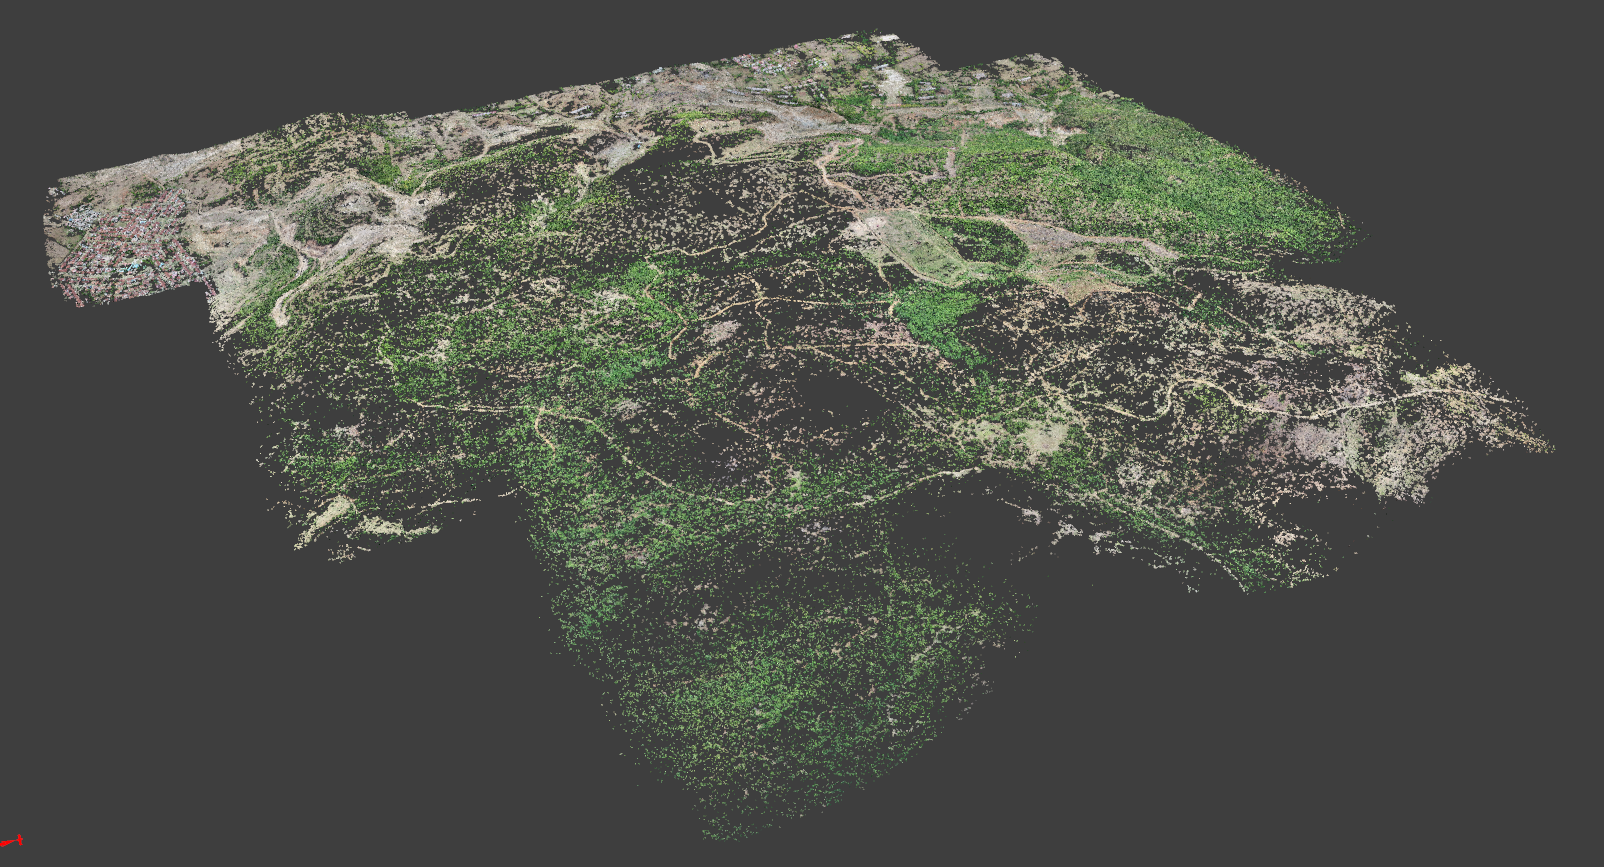
\includegraphics[width=1\linewidth]{image/initial processing.png}
    \caption{Hasil output dari proses initial processing}
    \label{hasil_initialprocessing}
\end{figure}

hasil ini akan menjadi dasar untuk tahap-tahap selanjutnya dalam pembuatan orthomosaik. Setelah Initial Processing selesai, pengguna dapat memeriksa hasil dan melakukan penyesuaian jika diperlukan sebelum melanjutkan ke tahap berikutnya seperti Point Cloud and Mesh, DSM, Orthomosaic and Index, dan sebagainya. Dalam penelitian ini, setelah melakukan initial processing, langkah selanjutnya yang krusial adalah penyesuaian dan penginputan Ground Control Point (GCP). Proses ini sangat penting untuk meningkatkan akurasi geometri dari model yang dihasilkan. GCP adalah titik-titik referensi di lapangan dengan koordinat yang diketahui secara akurat, yang digunakan untuk mengkalibrasi dan mengoreksi data pemetaan udara. Dengan memasukkan koordinat GCP yang tepat ke dalam software, kita dapat mengurangi kesalahan posisi dan meningkatkan ketelitian pemetaan secara keseluruhan. Hal ini memastikan bahwa hasil akhir pemetaan memiliki akurasi spasial yang tinggi dan dapat diandalkan untuk berbagai aplikasi. GCP yang digunakan juga sama seperti yang digunakan pada proses menggunakan Agisoft Metashape dan berjumlah 16 GCP. Distribusi spasial dari titik-titik GCP dapat dilihat pada Gambar \ref{penyebaran  pix}. Sementara itu, tahapan penyesuaian koordinat GCP terhadap citra drone diilustrasikan pada Gambar dan \ref{gcpakurat pix}, memberikan gambaran visual tentang proses penyelarasan yang dilakukan. 

\begin{figure} [H]
    \centering
    \frame{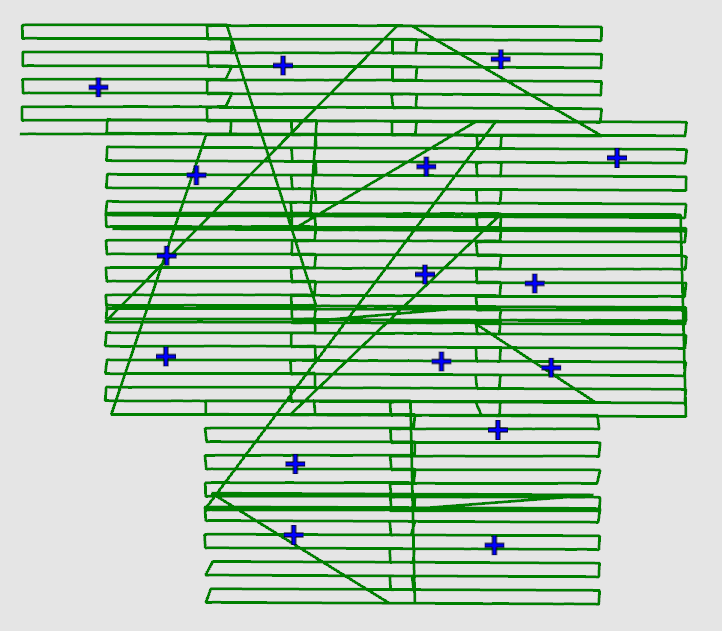
\includegraphics[width = 13cm]{image/penyebaran GCP.png}}
    \caption{Penyebaran titik Ground Control Point ditandai simbol (+).}
    \label{penyebaran pix}
\end{figure}

\begin{figure} [H]
    \centering
    \frame{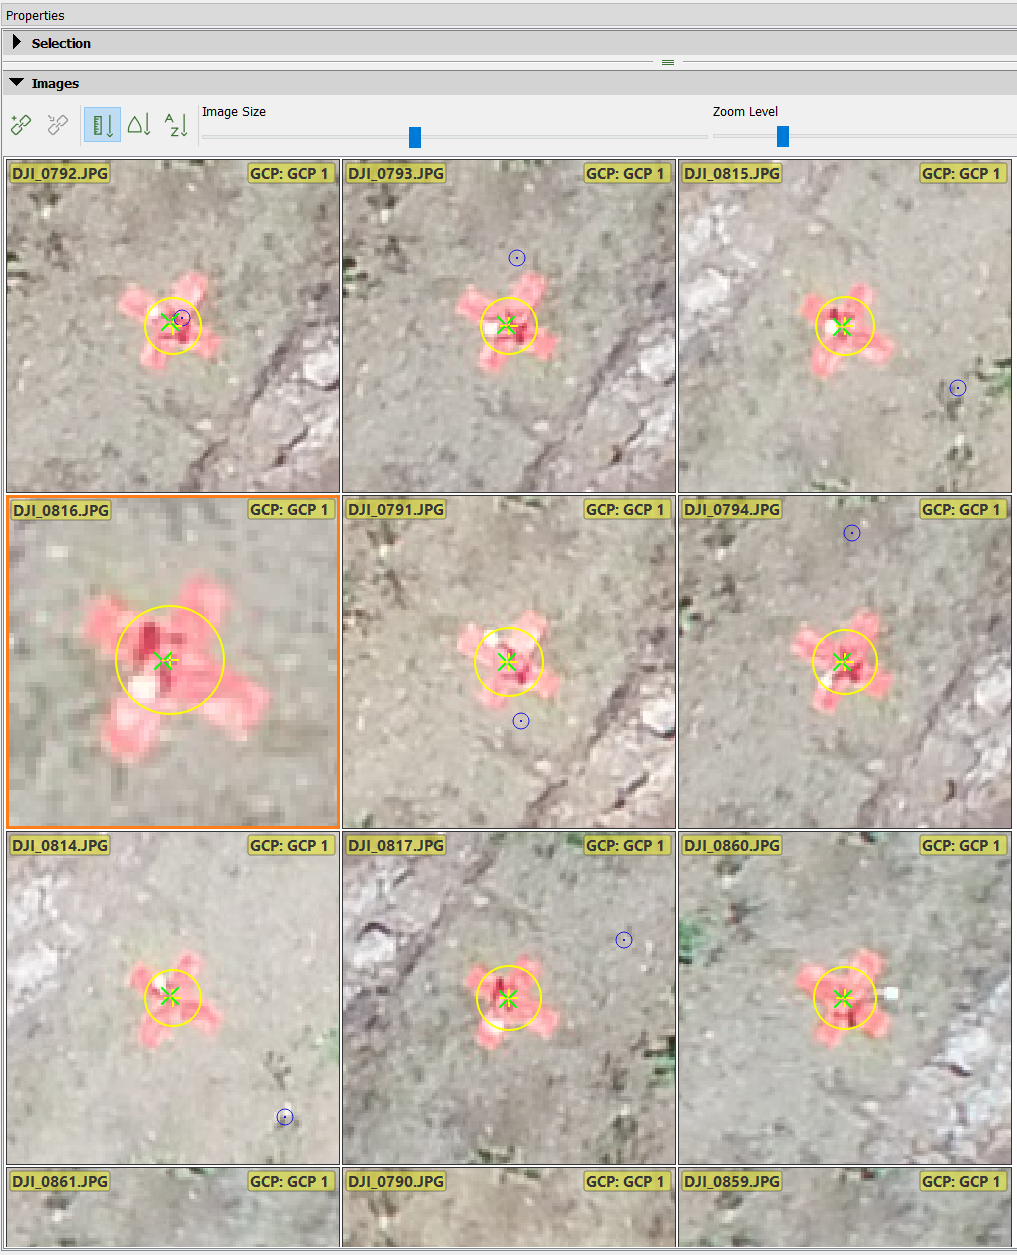
\includegraphics[width = 11.5cm]{image/penentuan GCP.png}}
    \caption{Proses penyesuaian Ground Control Point.}
    \label{gcpakurat pix}
\end{figure}

Tahap selanjutnya adalah Point Cloud and Mesh, sebuah proses terintegrasi dalam PIX4Dmapper yang memerlukan waktu lebih lama dan sumber daya perangkat keras yang intensif. Dalam tahap ini, perangkat lunak tidak hanya menghasilkan titik-titik 3D (point cloud) yang secara akurat merepresentasikan permukaan objek atau area lahan yang dipetakan, tetapi juga langsung menghasilkan mesh 3D. PIX4Dmapper memanfaatkan informasi dari foto-foto yang telah diproses sebelumnya untuk menentukan posisi 3D dari fitur-fitur yang terlihat pada setiap gambar dengan presisi tinggi. Hasil dari proses ini adalah kumpulan titik-titik padat yang mewakili struktur permukaan, serta mesh yang menghubungkan titik-titik tersebut menjadi model 3D yang solid. Tingkat kepadatan point cloud yang dihasilkan jauh lebih tinggi dibandingkan tie points pada tahap initial processing. Dalam penelitian ini, proses Point Cloud and Mesh memakan waktu sekitar 5 jam 37 menit dengan pengaturan kualitas Low (Fast), menghasilkan lebih dari 131 juta titik dan mesh yang sesuai. Penggabungan proses point cloud dan mesh ini memungkinkan PIX4Dmapper untuk menghasilkan model 3D yang lebih efisien dan siap digunakan. Visualisasi hasil dari tahap Point Cloud and Mesh dapat dilihat pada Gambar \ref{point cloud pix}, \ref{mesh pix}. Proses terintegrasi ini merupakan langkah penting dalam menghasilkan model 3D yang detail dan akurat untuk analisis lebih lanjut.

\begin{figure} [H]
    \centering
    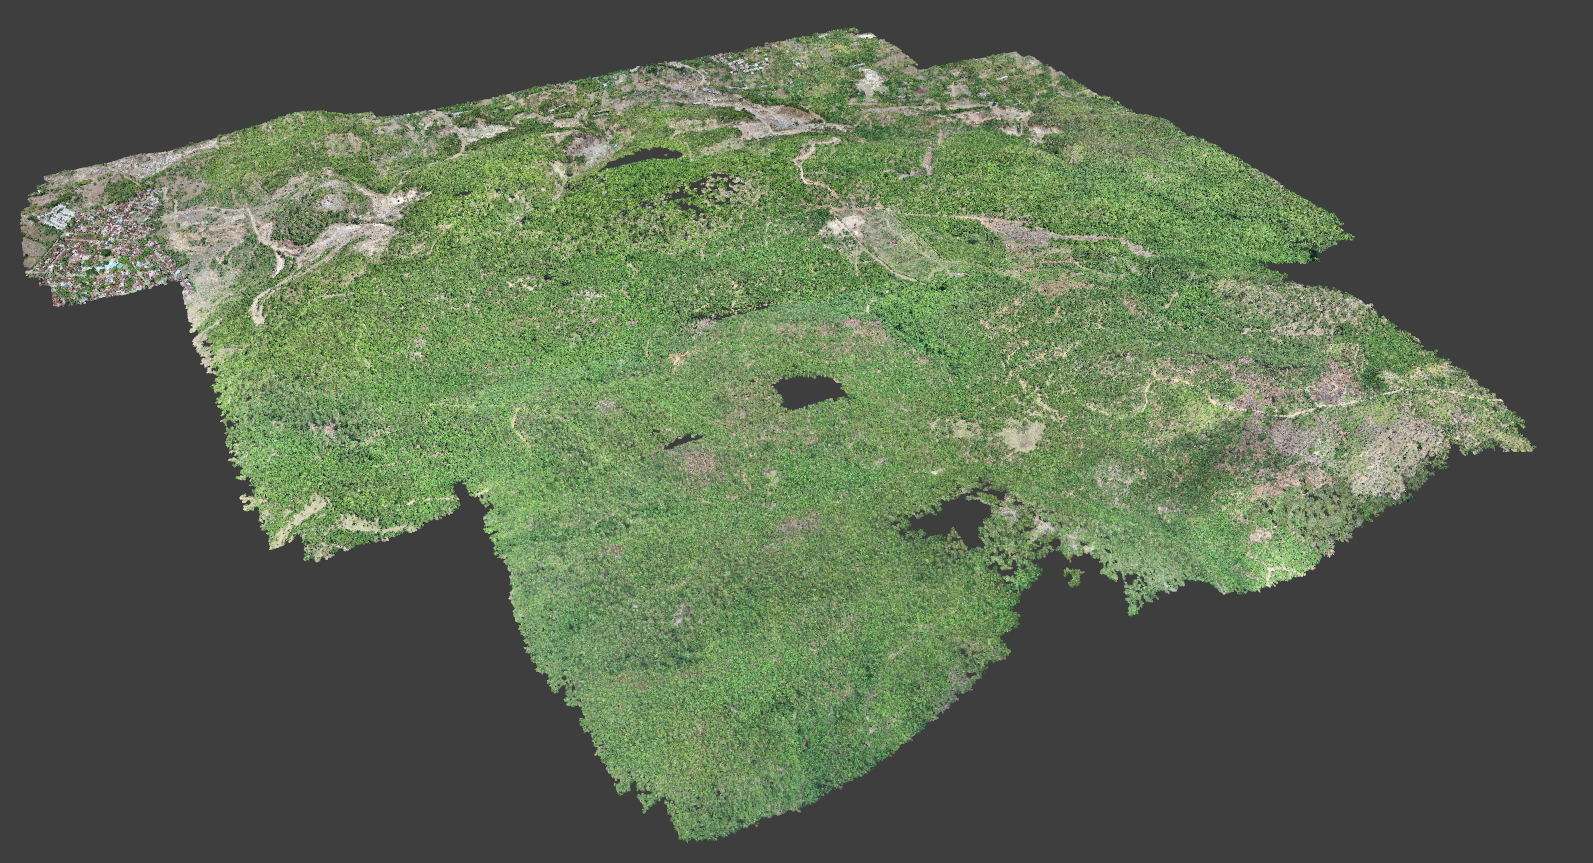
\includegraphics[width=1\linewidth]{image/point cloud.png}
    \caption{Hasil output dari proses point cloud}
    \label{point cloud pix}
\end{figure}

\begin{figure} [H]
    \centering
    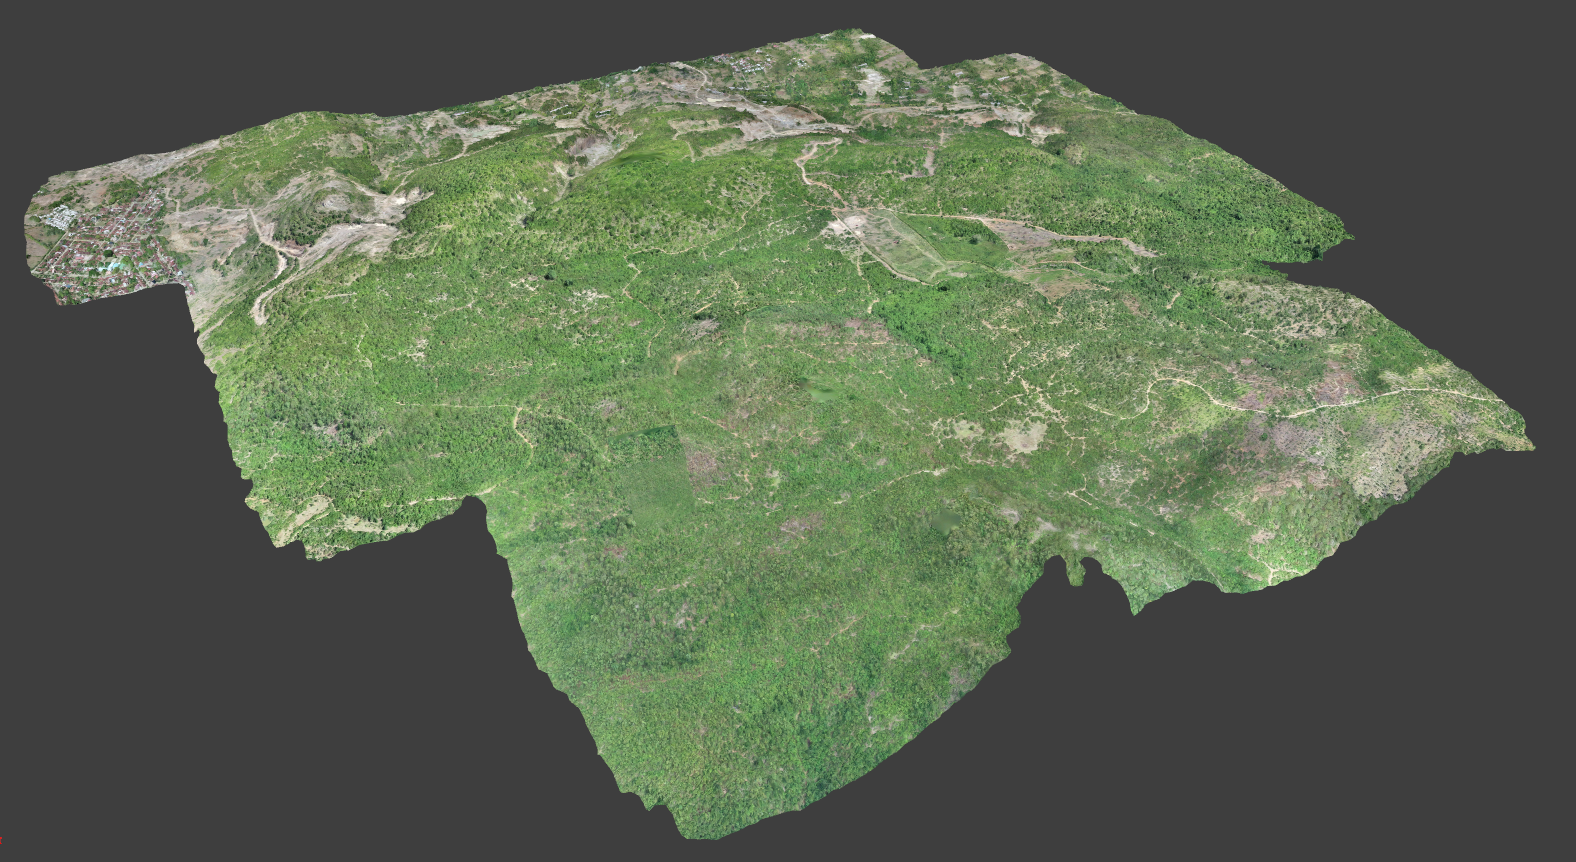
\includegraphics[width=1\linewidth]{image/mesh.png}
    \caption{Hasil output dari proses mesh}
    \label{mesh pix}
\end{figure}

Setelah proses pembuatan point cloud dan mesh selesai, perangkat lunak PIX4Dmapper akan melanjutkan ke tahap selanjutnya, yaitu pembuatan DSM (Digital Surface Model), dan orthomosaic.
Proses DSM menghasilkan model elevasi digital yang menggambarkan permukaan bumi termasuk semua objek di atasnya seperti bangunan dan vegetasi. DSM dibuat dengan menggunakan data ketinggian dari point cloud yang telah dihasilkan sebelumnya. Orthomosaic adalah citra foto udara yang telah dikoreksi secara geometris sehingga skala yang dihasilkan seragam dan dapat digunakan untuk pengukuran jarak dan luas yang akurat. Proses ini menggabungkan dan menyesuaikan berbagai foto udara menjadi satu citra yang detail dan tergeoreferensi. Hasil output dari proses DSM dan orthomosaic dapat dilihat pada Gambar \ref{dsm ortho}. DSM biasanya ditampilkan sebagai peta kontur atau visualisasi 3D berwarna, sementara orthomosaic akan terlihat seperti foto udara yang sangat detail dan akurat secara geometris dari area yang dipetakan.

\begin{figure} [H]
    \centering
    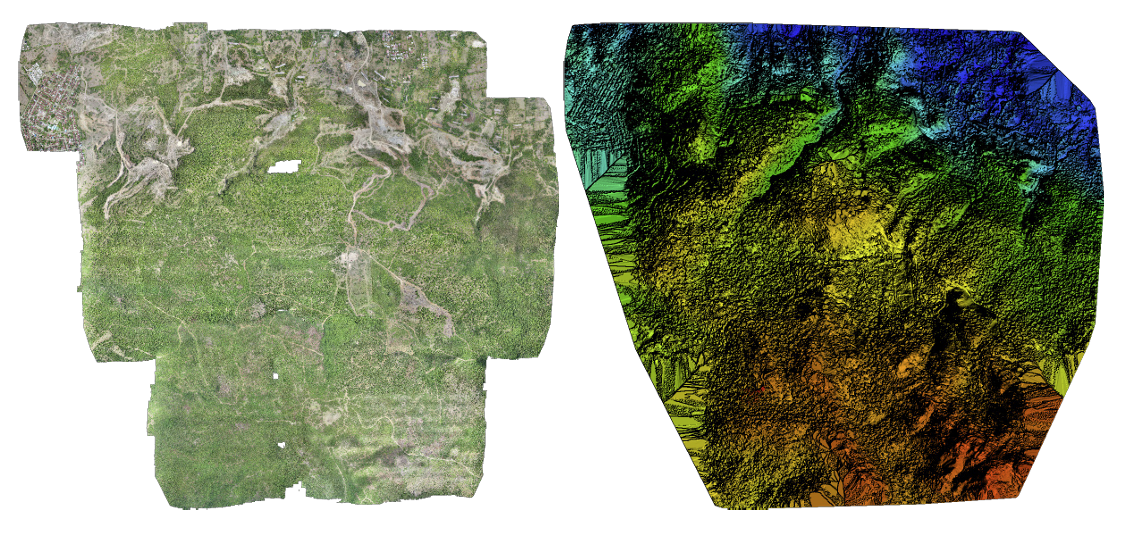
\includegraphics[width=1\linewidth]{image/DSM dan ortho.png}
    \caption{Hasil output DSM dan Orthomosaic}
    \label{dsm ortho}
\end{figure}

Hasil output orthomosaic dari perangkat lunak PIX4Dmapper mencapai resolusi yang sangat tinggi, yaitu 4,4 cm/pixel. Resolusi ini menunjukkan tingkat detail yang luar biasa dalam pemetaan menggunakan teknologi fotogrametri udara. Setiap pixel dalam citra orthomosaic mewakili area seluas 4,4 cm x 4,4 cm di permukaan bumi, memungkinkan identifikasi dan analisis objek-objek kecil dengan sangat jelas, seperti vegetasi individual, fitur-fitur arsitektur pada bangunan, infrastruktur jalan yang detail, dan objek-objek kecil di permukaan tanah. Pencapaian resolusi setinggi ini merupakan hasil dari kombinasi kualitas kamera drone yang digunakan, ketinggian terbang yang relatif rendah, tingkat overlap foto yang tinggi, serta kemampuan pengolahan canggih dari PIX4Dmapper. 

Berdasarkan serangkaian proses mosaik yang telah dilaksanakan menggunakan PIX4Dmapper, kita memperoleh beberapa hasil, salah satunya adalah orthomosaic. Dalam pelaksanaan proses mosaik menggunakan perangkat lunak PIX4Dmapper, terdapat beberapa pertimbangan dalam pemilihan pengaturan kualitas untuk mengoptimalkan hasil dan efisiensi waktu pemrosesan. Berikut ini, penulis akan memaparkan secara rinci mengenai proses, konfigurasi kualitas, serta durasi yang diperlukan untuk menjalankan setiap tahapan dalam PIX4Dmapper. Informasi tersebut dapat dilihat secara komprehensif pada Tabel \ref{runningpix}.

\begin{table}[h]
\centering
\caption{Ringkasan detail proses mosaik menggunakan PIX4Dmapper}
\begin{tabular}{|c|c|c|}
\hline
\textbf{Proses} & \textbf{Pengaturan kualitas} & \textbf{Waktu proses}\\
\hline
Initial Processing & Full & 4 jam 10 menit \\
\hline
Point Cloud & Low & 4 jam 46 menit \\
\hline
Build mesh & Medium & 51 menit \\
\hline
Build DSM & Sharp & 1 jam 22 menit \\
\hline
Build Orthomosaic & - & 5 jam 50 menit \\
\hline
\end{tabular}
\label{runningpix}
\end{table}

Data pada Tabel \ref{runningpix} menunjukkan kualitas tertinggi yang dapat diproses oleh spesifikasi komputer penulis menggunakan PIX4Dmapper. Upaya untuk menjalankan proses dengan kualitas yang lebih tinggi dapat mengakibatkan perangkat lunak mengeluarkan pesan kesalahan terkait memori tidak mencukupi ataupun perangkat lunak akan mengalami force close. Kesalahan ini dapat terjadi ketika perangkat lunak tidak mampu mengalokasikan jumlah memori yang diperlukan untuk menyelesaikan tugas.Perlu dicatat bahwa hal ini tidak selalu berarti total RAM yang terpasang pada sistem tidak cukup, melainkan lebih kepada jumlah RAM yang tersedia saat operasi tersebut dilakukan. Untuk data dalam tabel yang ditandai dengan simbol (-), hal ini menunjukkan penggunaan pengaturan default PIX4Dmapper atau penggunaan data olahan dari tahap sebelumnya tanpa opsi pengaturan tambahan. Berdasarkan analisis tabel tersebut, dapat disimpulkan bahwa untuk menjalankan proses mosaik menggunakan PIX4Dmapper dengan data foto udara pada penelitian ini membutuhkan waktu total selama 16 jam 59 menit. Waktu pemrosesan ini mencakup semua tahapan dari importasi gambar hingga generasi orthomosaic akhir. Sayangnya, pada hasil report dari aplikasi PIX4Dmapper tidak menyertakan informasi detail mengenai penggunaan RAM dan penyimpanan pada setiap prosesnya.

\begin{table}[H]
\centering
\renewcommand{\arraystretch}{1}
\caption{Nilai RMSE dari control point PIX4Dmapper}
\begin{tabular}{|l|r|r|r|r|r|}
\hline
\textbf{Label} &\textbf{ X error (cm)} &\textbf{ Y error (cm)} & \textbf{Z error (cm)} & \textbf{Total (cm)} \\
\hline
GCP 1 (3D) & -0.9 & -1.5 & -0.2 & 1.75 \\
\hline
GCP 2 (3D) & -0.5 & -1.0 & 0.3 & 1.15 \\
\hline
GCP 3 (3D) & -2.2 & 1.8 & 0.2 & 2.85 \\
\hline
GCP 5 (3D) & 5.6 & 7.6 & -1.6 & 9.65 \\
\hline
GCP 6 (3D) & -1.2 & 0.5 & -1.3 & 1.85 \\
\hline
GCP 7 (3D) & -1.4 & -3.2 & 0.2 & 3.50 \\
\hline
GCP 9 (3D) & -2.8 & -5.9 & 1.0 & 6.60 \\
\hline
GCP 10 (3D) & 5.6 & 10.3 & -0.9 & 11.75 \\
\hline
GCP 11 (3D) & -2.4 & -0.8 & 5.8 & 6.35 \\
\hline
GCP 13 (3D) & -0.1 & 12.7 & 2.3 & 12.90 \\
\hline
GCP 14 (3D) & -3.6 & -8.7 & -0.9 & 9.45 \\
\hline
GCP 15 (3D) & 2.8 & -1.7 & -2.5 & 4.10 \\
\hline
GCP 18 (3D) & 94.1 & -132.1 & -85.0 & 183.45 \\
\hline
GCP 19 (3D) & -0.8 & -0.3 & 2.9 & 3.05 \\
\hline
GCP 23 (3D) & 227.2 & -30.4 & -5.5 & 229.85 \\
\hline
GCP 24 (3D) & 1.8 & 1.9 & -0.3 & 2.60 \\
\hline
\textbf{RMS Error} & \textbf{61.5358} & \textbf{34.2995} & \textbf{21.3708} & \textbf{73.31} \\
\hline
\end{tabular}
\label{tab:gcp_error_cm}
\end{table}

Selain pengaturan kualitas dan efisiensi waktu, pada Tabel \ref{tab:gcp_error_cm} dapat dilihat hasil selanjutnya yang akan dipaparkan berkaitan dengan keakuratan geometri menggunakan Ground Control Points (GCP) dengan metode Root Mean Square Error (RMSE), yang memberikan gambaran kuantitatif mengenai presisi hasil mosaik. Analisis ini sangat penting untuk menilai kualitas dan keandalan peta yang dihasilkan. Dengan menggunakan titik-titik kontrol di lapangan (GCP) dan menghitung tingkat kesalahan (RMSE), dapat diketahui seberapa tepat gambar mosaik yang dihasilkan. Hal ini membantu dalam menentukan apakah hasil pemetaan sudah memenuhi standar untuk berbagai keperluan yang berbeda.

Berdasarkan hasil analisis pada Tabel 4.8, diperoleh gambaran komprehensif mengenai akurasi pengukuran. Total RMSE mencapai 73,31 cm, mencerminkan kesalahan gabungan dari semua arah. Kesalahan pada sumbu X (timur-barat) sebesar 61,5358 cm, sementara pada sumbu Y (utara-selatan) lebih rendah yaitu 34,2995 cm. Kesalahan vertikal atau Z error menunjukkan nilai terendah sebesar 21,3708 cm, mengindikasikan bahwa pengukuran ketinggian cenderung lebih presisi dibandingkan pengukuran horizontal. Dari data tersebut, dapat dihitung RMSEr (Root Mean Square Error radial) yang merepresentasikan kesalahan radial horizontal gabungan, yaitu sebesar 70,42 cm. Nilai ini diperoleh dari akar kuadrat jumlah kuadrat RMSE X dan Y. Secara keseluruhan, hasil ini menunjukkan bahwa pengukuran memiliki tingkat akurasi yang bervariasi dengan kisaran kesalahan yang cukup besar, terutama pada pengukuran horizontal. Terlihat adanya beberapa titik kontrol dengan error yang sangat tinggi, seperti GCP 23 (3D) dengan total error mencapai 229,85 cm, yang secara signifikan mempengaruhi nilai RMSE keseluruhan. Pengukuran vertikal menunjukkan konsistensi yang lebih baik dibandingkan pengukuran horizontal, namun masih terdapat ruang untuk peningkatan akurasi secara keseluruhan, terutama dalam mengurangi variasi error yang ekstrem pada beberapa titik kontrol.

Setelah memperoleh data RMSE dari proses mosaik, langkah berikutnya adalah menghitung nilai Circular Error (CE90) dan Linear Error (LE90). Perhitungan ini mengacu pada rumus yang diatur oleh Badan Informasi Geospasial tahun 2014. Hasil perhitungan ini dapat dilihat pada Tabel \ref{tab:hasil_perhitungan le}, yang memberikan gambaran tentang seberapa akurat data geospasial tersebut setelah proses mosaik.

\begin{table}[H]
\centering
\caption{Hasil Perhitungan RMSEr, RMSEz, CE90, dan LE90 pada perangkat lunak PIX4Dmapper}
\begin{tabular}{|l|c|}
\hline
\textbf{Komponen} & \textbf{Nilai (cm)} \\
\hline
RMSEr & 70.45 \\
RMSEz & 21,37 \\
CE90 & 106,91 \\
LE90 & 35,26 \\
\hline
\end{tabular}
\label{tab:hasil_perhitungan le}
\end{table}

\section{Analisis Perbandingan}

\par Setelah menyelesaikan proses mosaik menggunakan dua perangkat lunak berbeda, yakni Agisoft Metashape dan PIX4Dmapper, dengan dataset identik berupa 4.701 foto udara dan 16 titik koordinat GCP (Ground Control Points), langkah berikutnya adalah melakukan analisis komparatif terhadap hasil mosaik. Perbandingan ini akan berfokus pada beberapa aspek kunci, meliputi keakuratan geometri, resolusi spasial, efisiensi waktu pemrosesan, serta kualitas visual secara detail pada beberapa titik sampel orthomosaik. Analisis mendalam ini bertujuan untuk mengevaluasi kinerja kedua perangkat lunak dalam menghasilkan orthomosaik yang presisi dan berkualitas tinggi, sehingga dapat memberikan wawasan komprehensif mengenai keunggulan dan kelemahan masing-masing perangkat lunak dalam konteks pengolahan data foto udara.

\subsection{Akurasi Geometri}

Berdasarkan Tabel \ref{tab:perbandingan} yang menunjukkan perbandingan hasil perhitungan RMSEr, RMSEz, CE90, dan LE90 pada perangkat lunak Agisoft PIX4Dmapper dan Agisoft Metashape dalam satuan sentimeter (cm), dapat disimpulkan:
PIX4Dmapper masih menghasilkan nilai kesalahan yang lebih tinggi dibandingkan Agisoft Metashape untuk semua parameter. RMSEr PIX4Dmapper (70,45 cm) lebih besar daripada Metashape (9,17 cm). Pola yang sama terlihat untuk RMSEz, CE90, dan LE90.

\begin{table}[H]
\centering
\begin{tabular}{|l|c|c|}
\hline
\textbf{Komponen} & \textbf{Agisoft Metashape (cm)} & \textbf{PIX4Dmapper (cm)} \\
\hline
RMSEr  & 9,17 & 70,45 \\
RMSEz  & 8,66 & 21,37 \\
CE90  & 13,92 & 106,91 \\
LE90  & 14,29 & 35,26 \\
\hline
\end{tabular}
\caption{Perbandingan Hasil Perhitungan RMSEr, RMSEz, CE90, dan LE90 pada Perangkat Lunak Agisoft PIX4Dmapper dan Agisoft Metashape}
\label{tab:perbandingan}
\end{table}

Berdasarkan perbandingan nilai CE90 dan LE90 yang dihasilkan oleh Agisoft Metashape dan PIX4Dmapper dengan standar ketelitian peta RBI, dapat disimpulkan bahwa kedua perangkat lunak mampu menghasilkan mosaik dengan ketelitian tinggi. Agisoft Metashape menunjukkan performa yang sangat baik dengan nilai CE90 13,92 cm dan LE90 14,29 cm, sementara PIX4Dmapper menghasilkan nilai CE90 106,91 cm dan LE90 35,26 cm. Ketika dibandingkan dengan Tabel 2.2 Ketelitian Peta RBI, kedua hasil ini menunjukkan potensi untuk memenuhi standar ketelitian pada skala peta yang berbeda.

\begin{itemize}
    \item \textbf{Agisoft Metashape:} Mampu mencapai ketelitian peta RBI untuk skala 1:1.000 kelas 1. Nilai CE90 dan LE90 yang dihasilkan bahkan lebih baik dari batas maksimum yang ditetapkan untuk skala ini (0,2 m untuk keduanya), menunjukkan potensi untuk ketelitian pada skala yang lebih besar jika standar tersedia.
    \item \textbf{PIX4Dmapper:} Dapat mencapai ketelitian peta RBI untuk skala 1:2.500 kelas 1. Hasil ini memenuhi dengan baik standar yang ditetapkan untuk skala tersebut, di mana batas maksimum CE90 dan LE90 adalah 0,5 m.
\end{itemize}

Ketelitian peta RBI tertinggi yang dapat dicapai berdasarkan hasil mosaik adalah skala 1:1.000 kelas 1 untuk Agisoft Metashape, dengan potensi untuk skala yang lebih besar, dan skala 1:2.500 kelas 1 untuk PIX4Dmapper. Kedua perangkat lunak menghasilkan mosaik yang memenuhi standar ketelitian tinggi untuk pemetaan RBI, dengan Agisoft Metashape menunjukkan keunggulan dalam mencapai ketelitian untuk skala peta yang lebih besar.

\subsection{Resolusi}

hasil orthomosaik dari kedua perangkat lunak menunjukkan resolusi yang sangat tinggi, dengan PIX4Dmapper menghasilkan resolusi yang sedikit lebih tinggi dibandingkan Agisoft Metashape. Orthomosaik yang dihasilkan oleh PIX4Dmapper memiliki resolusi 77405x69710 piksel, sementara Agisoft Metashape menghasilkan resolusi 75364x67824 piksel. Perbedaan ini menunjukkan bahwa PIX4Dmapper mampu menghasilkan citra dengan detail yang sedikit lebih tinggi, dengan selisih sekitar 2041 piksel pada dimensi panjang dan 1886 piksel pada dimensi lebar. Meskipun perbedaan ini ada, kedua hasil dapat dianggap memiliki kualitas resolusi yang sangat baik untuk keperluan pemetaan dan analisis spasial yang membutuhkan tingkat detail tinggi. Perbedaan resolusi ini mungkin tidak signifikan untuk sebagian besar aplikasi praktis, namun dapat menjadi pertimbangan dalam proyek-proyek yang memerlukan tingkat presisi yang sangat tinggi.

Begitu pula terkait ground resolution dari hasil pemrosesan Agisoft Metashape menunjukkan ground resolution sebesar 4,54 cm/pixel, sedangkan Pix4Dmapper menghasilkan 4,4 cm/pixel. Perbedaan ini menunjukkan bahwa secara umum, Pix4Dmapper berhasil menghasilkan detail yang sedikit lebih halus pada permukaan objek yang dipetakan dibandingkan dengan Agisoft Metashape. Namun, perbedaan sebesar 0,14 cm/pixel ini relatif kecil dan mungkin tidak terlalu signifikan secara visual, terutama jika dilihat pada skala yang lebih besar.

\subsection{Waktu Pemrosesan}

Setelah selesai melakukan proses mosaik pada kedua perangkat lunak, yaitu Agisoft Metashape dan PIX4Dmapper berdasarkan pengaturan kualitas masing-masing, maka diperoleh data waktu yang dibutuhkan untuk setiap tahap proses pada kedua aplikasi, seperti yang terlihat pada Tabel 4.11 berikut.

\begin{table}[h]
\centering
\caption{Perbandingan Proses, Waktu, dan Kualitas antara Agisoft Metashape dan PIX4Dmapper}
\begin{tabular}{|l|c|c|c|c|}
\hline
\multirow{2}{*}{Proses} & \multicolumn{2}{c|}{Agisoft Metashape} & \multicolumn{2}{c|}{PIX4Dmapper} \\
\cline{2-5}
 & Kualitas & Waktu & Kualitas & Waktu \\
\hline
Initial Processing & High & 1 jam 12 menit & Full & 4 jam 10 menit \\
\hline
Point Cloud & High & 13 jam 48 menit & Low & 4 jam 46 menit \\
\hline
Build Model / mesh & Medium & 3 jam 17 menit & Medium & 51 menit \\
\hline
Build Texture & - & 5 jam 52 menit & - & - \\
\hline
Build DEM / DSM & Ultra High & 9 menit & Sharp & 1 jam 22 menit \\
\hline
Build Orthomosaic & - & 2 jam 48 menit & - & 5 jam 50 menit \\
\hline
\end{tabular}
\label{tab:perbandinganwaktu}
\end{table}

Berdasarkan Tabel \ref{tab:perbandinganwaktu
}, dapat disimpulkan bahwa Agisoft Metashape dan PIX4Dmapper memiliki karakteristik pemrosesan yang berbeda. Meskipun pada pandangan pertama Agisoft Metashape tampak memerlukan waktu pemrosesan yang lebih panjang secara keseluruhan, penting untuk mempertimbangkan bahwa durasi pemrosesan sangat dipengaruhi oleh pengaturan kualitas yang dipilih sebelum proses dimulai. Analisis lebih mendalam menunjukkan bahwa dalam beberapa tahapan dengan pengaturan kualitas yang setara, Agisoft Metashape justru mengungguli PIX4Dmapper dalam hal efisiensi waktu. Sebagai contoh, pada tahap Initial Processing, Build DEM dan Orthomosaic, Agisoft Metashape menyelesaikan tugas jauh lebih cepat dibandingkan PIX4Dmapper. Di sisi lain, PIX4Dmapper menunjukkan keunggulan signifikan dalam proses pembangunan mesh, dengan waktu pemrosesan yang jauh lebih singkat dibandingkan Agisoft Metashape. Hal ini menggambarkan bahwa masing-masing software memiliki kekuatan tersendiri dalam aspek-aspek tertentu dari alur kerja fotogrametri.

\subsection{Kualitas Visual}

Analisis krusial dalam proses mosaik pada penelitian ini adalah perbandingan hasil visual dari kedua perangkat lunak. Tahap ini melibatkan pengambilan beberapa sampel gambar dari orthomosaik yang dihasilkan oleh kedua perangkat lunak di berbagai lokasi yang berbeda. Lokasi-lokasi yang dipilih mencakup komplek perumahan, jalan, lereng perbukitan, dan hutan dengan vegetasi lebat. Pemilihan lokasi yang beragam ini bertujuan untuk mengevaluasi kinerja perangkat lunak dalam menangani berbagai jenis terrain dan fitur permukaan. Hasil perbandingan visual ini disajikan secara komprehensif dalam Gambar 4.18, 4.19, 4.20, dan 4.21. Melalui analisis ini, dapat diperoleh pemahaman mendalam tentang kualitas dan akurasi orthomosaik yang dihasilkan oleh masing-masing perangkat lunak dalam berbagai kondisi lapangan.

\begin{figure} [H]
    \centering
    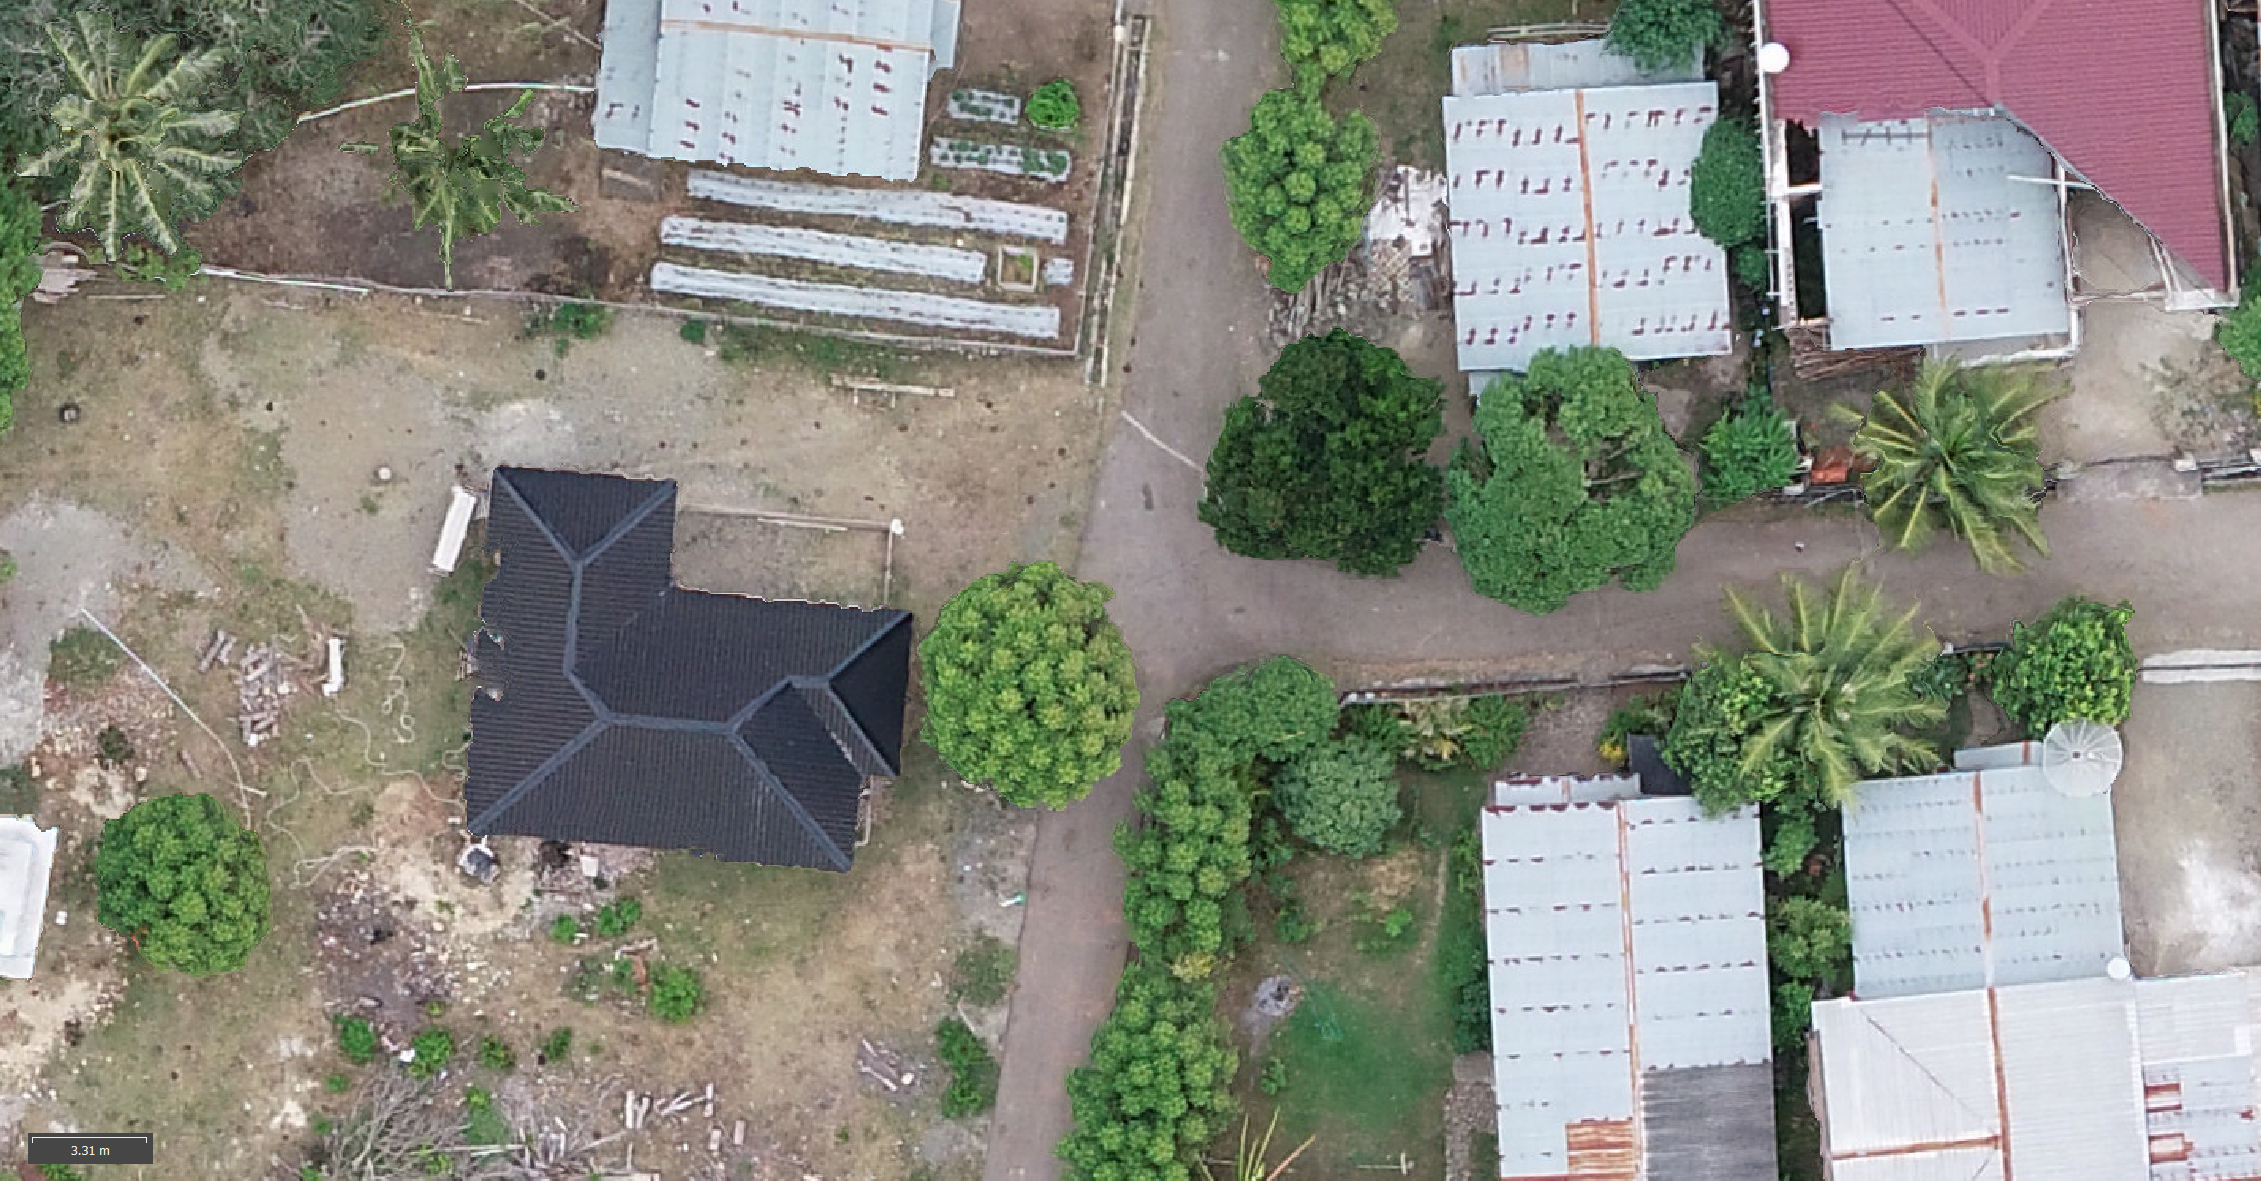
\includegraphics [width=1\linewidth]{image/agisoft perumahan.png}
    \caption{Hasil mosaik Agisoft Metashape di area perumahan}
    \label{visual perumahan 1}
\end{figure}

\begin{figure} [H]
    \centering
    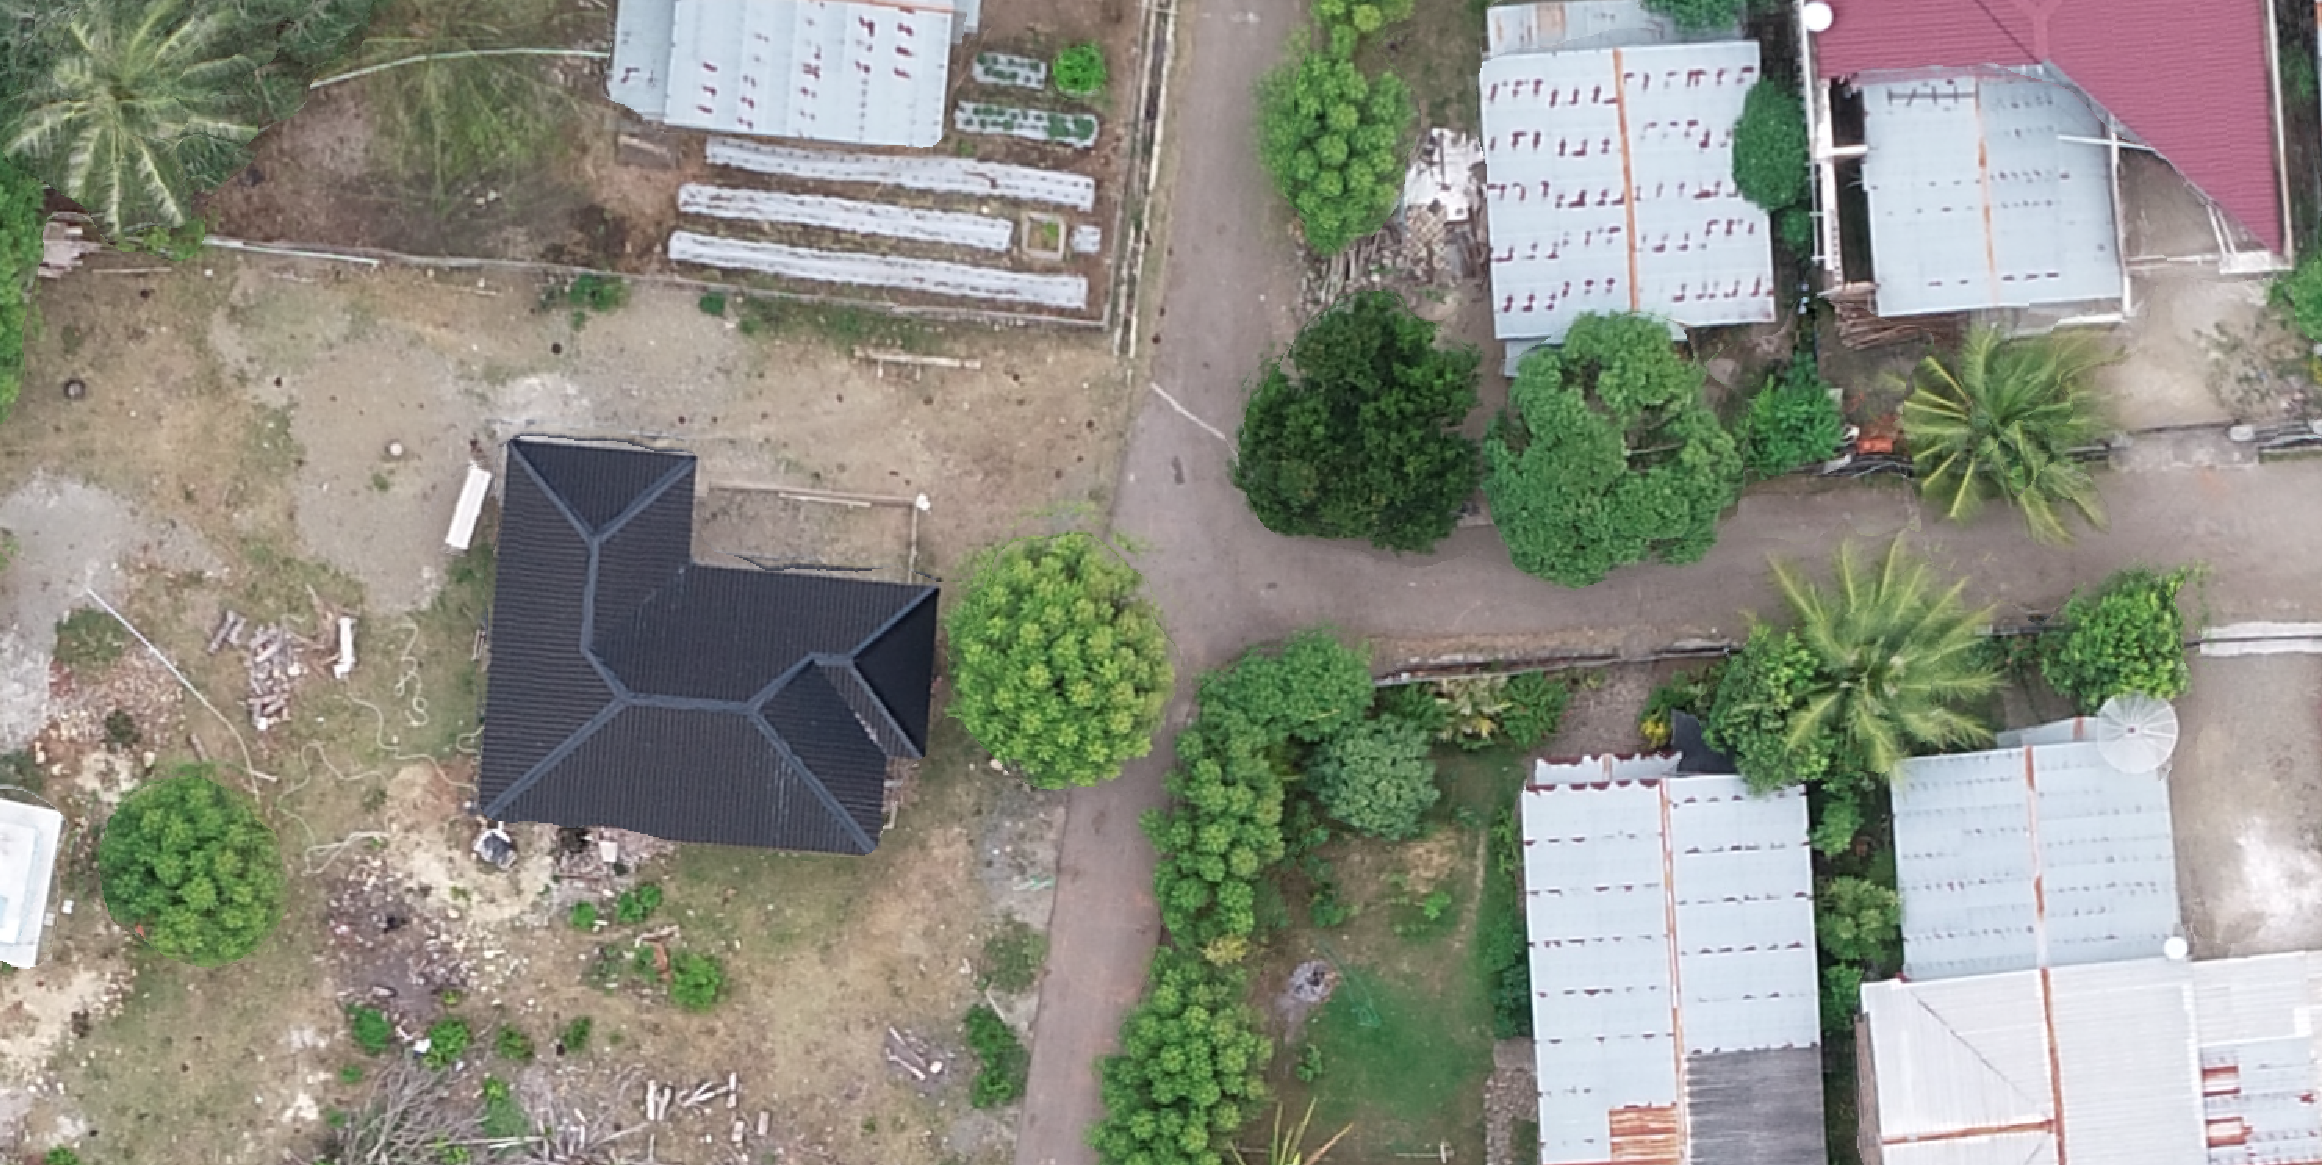
\includegraphics [width=1\linewidth]{image/pix perumahan.png}
    \caption{Hasil mosaik PIX4Dmapper di area perumahan}
    \label{visual perumahan 2}
\end{figure}

Dalam perbandingan hasil pengolahan citra mosaik di kawasan perumahan seperti pada Gambar \ref{visual perumahan 1} dan \ref{visual perumahan 2}, PIX4D Mapper menunjukkan keunggulan dibandingkan dengan Agisoft Metashape. Hasil dari Agisoft Metashape memperlihatkan beberapa kekurangan, terutama pada bagian ujung dan tepian atap rumah yang tampak bergerigi. Sebaliknya, PIX4D Mapper mampu menghasilkan rekonstruksi tepian atap dengan presisi tinggi dan detail yang sangat baik. Perlu dicatat bahwa perbedaan kualitas ini hanya terlihat pada beberapa area rumah tertentu, bukan pada keseluruhan citra.


\begin{figure} [H]
    \centering
    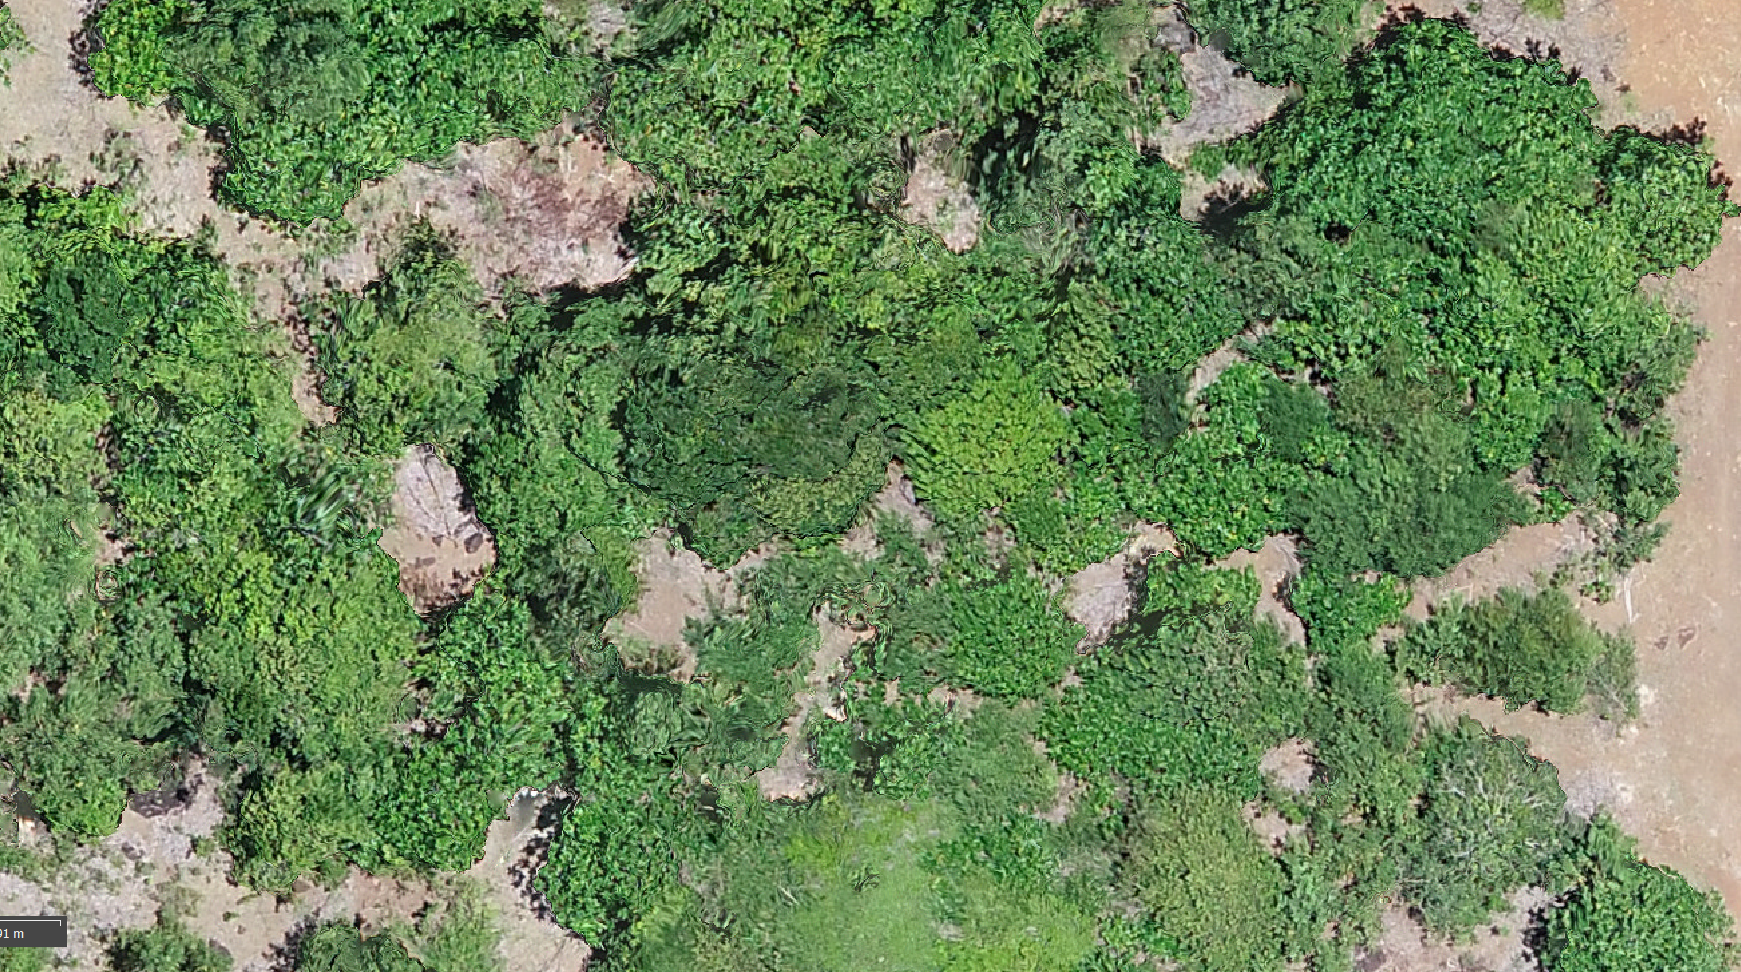
\includegraphics [width=1\linewidth]{image/agisoft vegetasi.png}
    \caption{Hasil mosaik Agisoft Metashape di area vegetasi}
    \label{visual vegetasi 1}
\end{figure}

\begin{figure} [H]
    \centering
    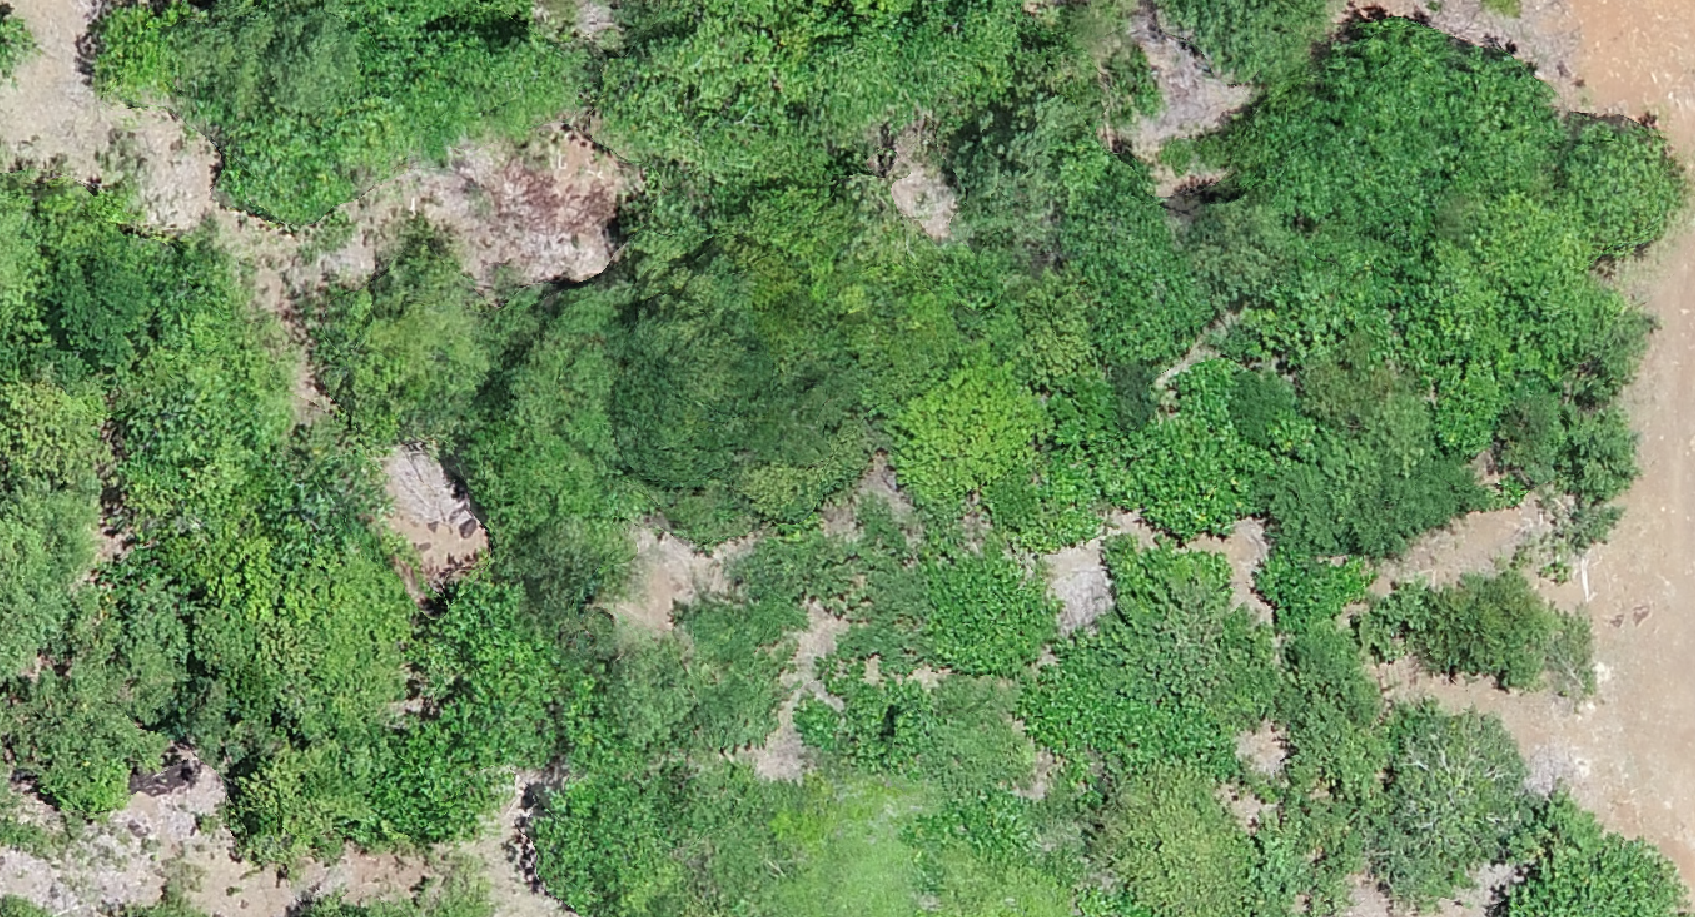
\includegraphics [width=1\linewidth]{image/pix vegetasi.png}
    \caption{Hasil mosaik PIX4Dmapper di area vegetasi}
    \label{visual vegetasi 2}
\end{figure}

Dalam perbandingan area vegetasi, Agisoft Metashape menghasilkan gambar yang lebih tajam, sementara PIX4D Mapper menghasilkan citra yang lebih halus. Meski demikian, hasil Agisoft Metashape menunjukkan beberapa kelemahan, seperti pohon yang tampak kabur dan daun yang menyatu. Pada hasil PIX4D Mapper, walaupun kurang tajam dalam detail namun berhasil memproses vegetasi secara lebih konsisten. Kedua perangkat lunak ini memiliki kelebihan dan kekurangan masing-masing dalam memvisualisasikan area bervegetasi.

\begin{figure} [H]
    \centering
    \includegraphics [width=1\linewidth]{image/lereng perbukitan agisoft.png}
    \caption{Hasil mosaik Agisoft Metashape di area lereng bukit}
    \label{visual lereng 1}
\end{figure}

\begin{figure} [H]
    \centering
    \includegraphics [width=1\linewidth]{image/lereng perbukitan pix.png}
    \caption{Hasil mosaik PIX4Dmapper di area lereng bukit}
    \label{visual lereng 2}
\end{figure}

Pada hasil mosaik di area lereng perbukitan, seperti yang ditunjukkan pada gambar \ref{visual lereng 1} dan \ref{visual lereng 2}, terlihat bahwa hasil dari Agisoft Metashape mengalami perubahan warna dan cahaya mendadak sehingga gambar tampak tidak menyatu. Sebaliknya, hasil dari PIX4D menunjukkan pengolahan gambar yang sangat baik tanpa ada masalah, menghasilkan mosaik yang lebih bagus dan konsisten.

\begin{figure} [H]
    \centering
    \includegraphics [width=1\linewidth]{image/jalan agisoft.png}
    \caption{Hasil mosaik Agisoft Metashape di area perkebunan}
    \label{visual jalan 1}
\end{figure}

\begin{figure} [H]
    \centering
    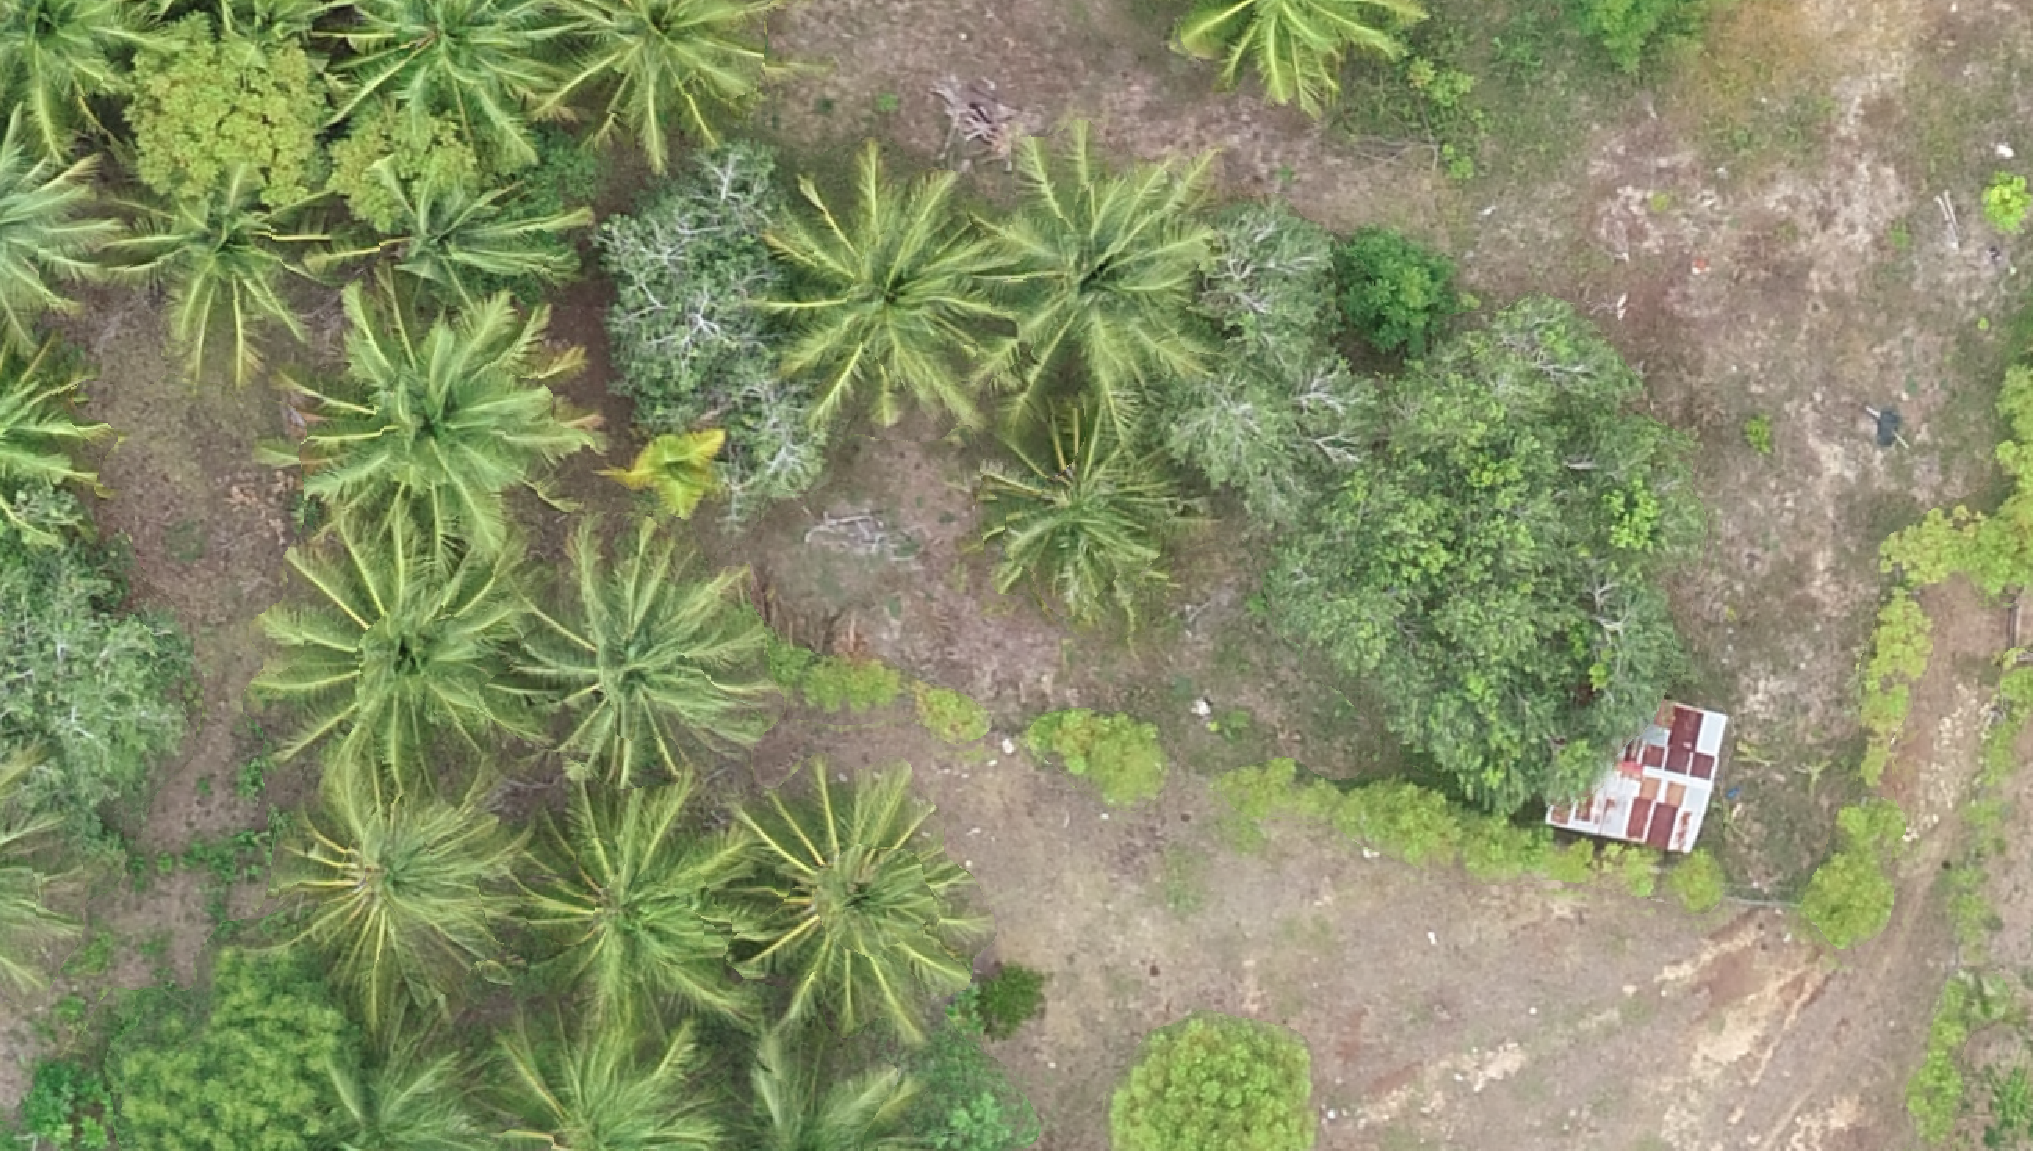
\includegraphics [width=1\linewidth]{image/jalan pix.png}
    \caption{Hasil mosaik PIX4Dmapper di area perkebunan}
    \label{visual jalan 2}
\end{figure}

Hasil mosaik pada area perkebunan, seperti yang terlihat pada Gambar \ref{visual jalan 1} dan \ref{visual jalan 2}, menunjukkan bahwa kedua perangkat lunak, Agisoft Metashape dan PIX4D Mapper, mampu menghasilkan gambar permukaan tanah dengan baik. Namun, keduanya menghadapi kesulitan dalam memproses bagian pohon kelapa, sehingga masih terdapat beberapa kekurangan pada hasil akhir.

\begin{figure} [H]
    \centering
    \includegraphics [width=1\linewidth]{image/bolong agisoft.png}
    \caption{Hasil mosaik Agisoft Metashape berlubang di area data yang rusak}
    \label{visual bolong 1}
\end{figure}

\begin{figure} [H]
    \centering
    \includegraphics [width=1\linewidth]{image/bolong pix.png}
    \caption{Hasil mosaik PIX4Dmapper berlubang di area data yang rusak}
    \label{visual bolong 2}
\end{figure}

Selain perbandingan visual, seperti yang terlihat pada Gambar \ref{visual bolong 1} dan \ref{visual bolong 2} terdapat data foto udara yang diduga rusak dan tidak dapat dikalibrasi selama proses pengaturan foto di kedua perangkat lunak. Kerusakan ini menyebabkan hilangnya foto udara di area tertentu, mengakibatkan adanya lubang pada hasil mosaik. Satu-satunya cara untuk memperbaiki data yang rusak ini adalah dengan mengambil ulang foto udara menggunakan drone di area yang sama
% Baris ini digunakan untuk membantu dalam melakukan sitasi
% Karena diapit dengan comment, maka baris ini akan diabaikan
% oleh compiler LaTeX.
\begin{comment}
\bibliography{daftar-pustaka}
\end{comment}